\documentclass[]{formalLabReport}

\usepackage{graphicx}

\usepackage{tikz}

%%%%%%%%%%%%%%%%%%%%%%%%%%%%%%%%%%%%%%%%%%%%%%%%%%%%%%%%%%%%%%%%%%%%%%
% LaTeX Overlay Generator - Annotated Figures v0.0.1
% Created with http://ff.cx/latex-overlay-generator/
% If this generator saves you time, consider donating 5,- EUR! :-)
%%%%%%%%%%%%%%%%%%%%%%%%%%%%%%%%%%%%%%%%%%%%%%%%%%%%%%%%%%%%%%%%%%%%%%
%\annotatedFigureBoxCustom{bottom-left}{top-right}{label}{label-position}{box-color}{label-color}{border-color}{text-color}
\newcommand*\annotatedFigureBoxCustom[8]{\draw[#5,thick,rounded corners] (#1) rectangle (#2);\node at (#4) [fill=#6,thick,shape=circle,draw=#7,inner sep=2pt,font=\sffamily,text=#8] {\textbf{#3}};}
%\annotatedFigureBox{bottom-left}{top-right}{label}{label-position}
\newcommand*\annotatedFigureBox[4]{\annotatedFigureBoxCustom{#1}{#2}{#3}{#4}{white}{white}{black}{black}}
\newcommand*\annotatedFigureText[4]{\node[draw=none, anchor=south west, text=#2, inner sep=0, text width=#3\linewidth,font=\sffamily] at (#1){#4};}
\newenvironment {annotatedFigure}[1]{\centering\begin{tikzpicture}
\node[anchor=south west,inner sep=0] (image) at (0,0) { #1};\begin{scope}[x={(image.south east)},y={(image.north west)}]}{\end{scope}\end{tikzpicture}}
%%%%%%%%%%%%%%%%%%%%%%%%%%%%%%%%%%%%%%%%%%%%%%%%%%%%%%%%%%%%%%%%%%%%%%


\graphicspath{ {./report-images/} }
\begin{document}

\title{Electronics Online Challenge}
\author{Raider Robotics - MSOE1}
\submissionDate{12/7/2020}

\maketitle

\tableofcontents

\newpage

\section{Introduction}
For this challenge, we chose to disassemble a Segway i2 SE PT. One of our teammates obtained 
the Segway in non-working condition and is currently trying to rebuild the electronics to add
features to the device. We decided that this challenge would provide an excellent opportunity for
us to gain a much better understanding to the proprietary systems inside of the device, and understand
the engineering that makes the devices as robust as they are.

\section{Component Summary}

\begin{center}
    \begin{table}[]
        \begin{tabular}{|l|l|l|l|l|l|}
        \hline
        Ref \#& Chip Identifier     & Description                & Documentation & Quantity \\ \hline
        1     & 16126797 AU195 02   &                            & Not Found     & 1        \\ \hline
        2     & 24C04WQ K525W       & I2C Bus EEPROM             & Actual        & 2        \\ \hline
        3     & 37021 58M C66L      &                            & Not Found     & 1        \\ \hline
        4     & 37021 58MCD29       &                            & Not Found     & 2        \\ \hline
        5     & 431AV PAHF          &                            & Not Found     & 1        \\ \hline
        6     & 55 84 K0            &                            & Not Found     & 1        \\ \hline
        7     & 56A504M HCT04       & Hex Inverter               & Similar       & 2        \\ \hline
        8     & 56A5NLM HCT4051M    & Demultiplexer              & Actual        & 3        \\ \hline
        9     & 59A2VHM TLC2254     & Op Amp                     & Actual        & 2        \\ \hline
        10    & 66C1HCM HCT4053M    & Multiplexer                & Similar       & 1        \\ \hline
        11    & 7438 543C G68V      &                            & Not Found     & 1        \\ \hline
        12    & 8L05A POIB8         & Positive Voltage Regulator & Similar       & 2        \\ \hline
        13    & A 7840 0611         & Isolation Amplifier        & Similar       & 4        \\ \hline
        14    & A82C250 4R4T0 n5064 &                            & Not Found     & 1        \\ \hline
        15    & BL05A POIB8         &                            & Not Found     & 2        \\ \hline
        16    & CHAQ LMC64 82AIM    & Operational Amplifier      & Actual        & 1        \\ \hline
        17    & CRLNLMG1 32B1M      &                            & Not Found     & 3        \\ \hline
        18    & IR 2136S 0515       & Three-phase MOSFET Driver  & Actual        & 2        \\ \hline
        19    & IRFP250N G3 DB      & N-Channel Power MOSFET     & Actual        & 12       \\ \hline
        20    & K0204 FQA 70N15     & N-Channel QFET MOSFET      & Actual        & 1        \\ \hline
        21    & K537 TOP414G 35721A & DC/DC PWM Switch           & Actual        & 1        \\ \hline
        22    & P185B MM74HCT 244WM & Octal 3-State Buffer       & Actual        & 1        \\ \hline
        23    & P56AB 98752         &                            & Not Found     & 1        \\ \hline
        24    & PVI 1050 NS 0538I4N & Photovoltaic Isolator      & Actual        & 1        \\ \hline
        25    & TMS 320LF2406APZA   & DSP Controller             & Not Found     & 1        \\ \hline
        \end{tabular}
    \end{table}
\end{center}

\section{Findings}
The Segway contains two main processing boards, which are identical mirrors. The processing board was
originally covered in a waterproof conformal coating to protect the electronics, which we removed selectively.
We found an array of chips and other components, and will attempt to classify them according to 
documentation for the component, or similar components with the same package type and similar IDs. 

While there is little documentation about the internals and processing systems of the Segway device, we found
groupings of similar components around specific parts of the board.

Talk about the importance of the components in the system.

\subsection{Battery Connector Proximity}
Signal processing components were found surrounding the battery connector on the bottom of the board.
There are three demultiplexer chips (Ref \# 8) surrounding the connector, which has four primary power pins
and eight signal pins (staggered pattern above and below). We have found some documentation for handling the
I2C communications being sent from the batteries, and we assume these demultiplexers are used to decode this
data for use on the board.

\section{Conclusion} 

\begin{figure}
    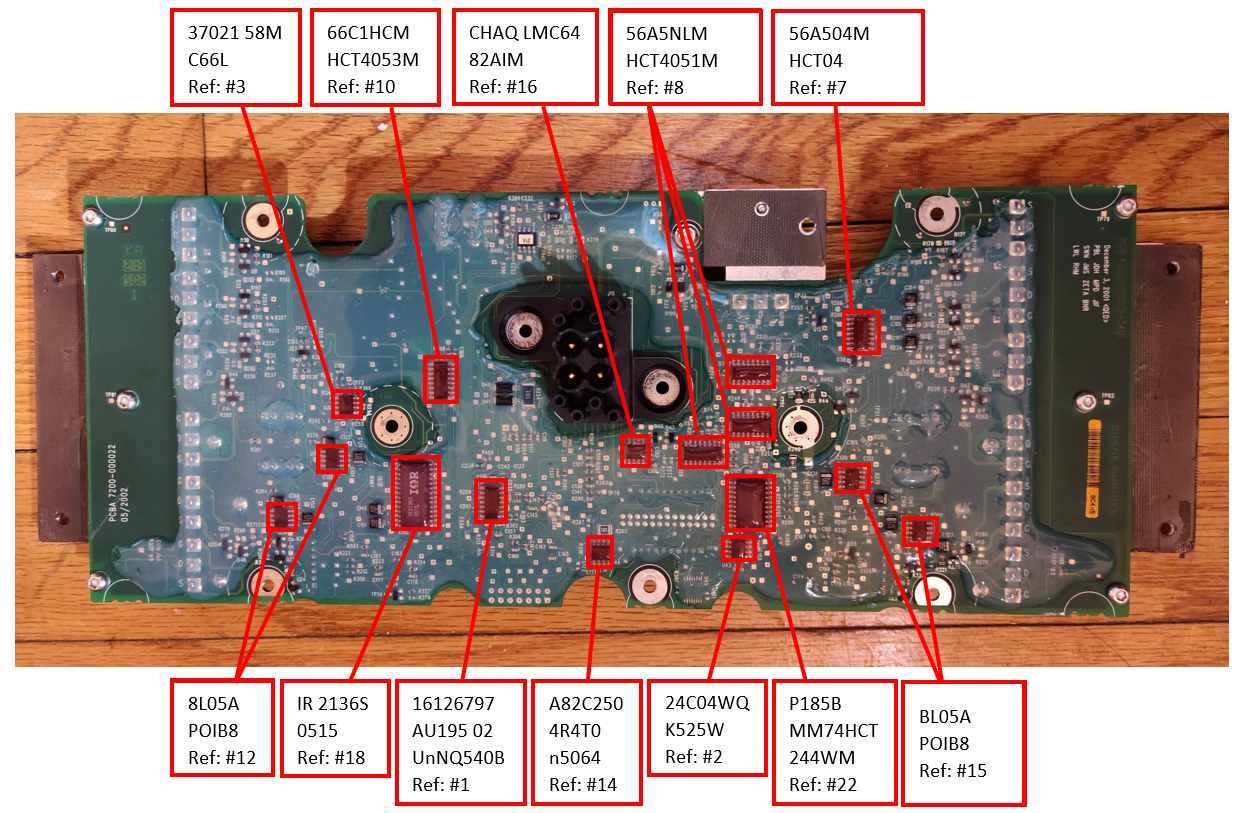
\includegraphics[]{annotatedBoardBack.png}
    \caption{caption}
    \label{fig:annotatedBoardBack.png}
\end{figure}

\begin{figure}
    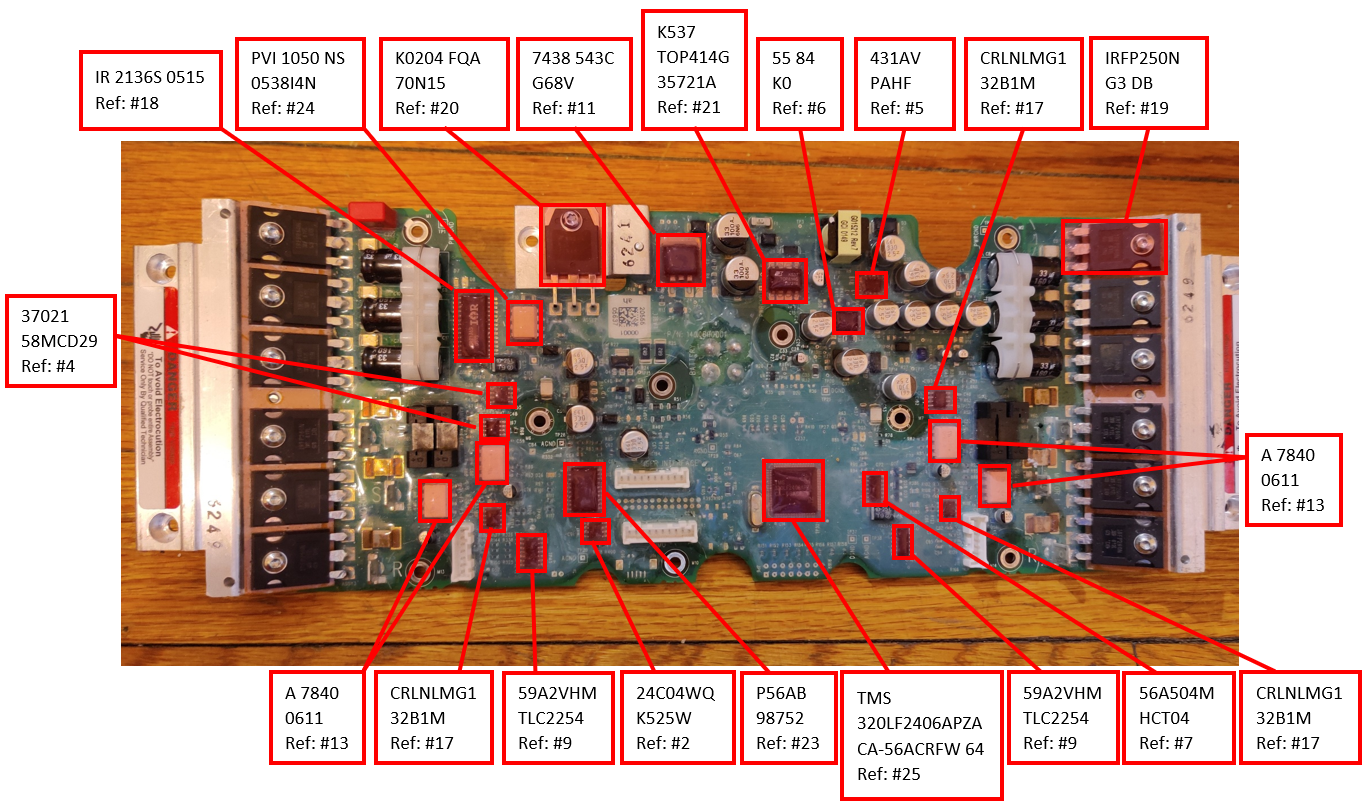
\includegraphics[]{annotatedBoardFront.png}
    \caption{caption}
    \label{fig:annotatedBoardFront.png}
\end{figure}

\begin{figure}
    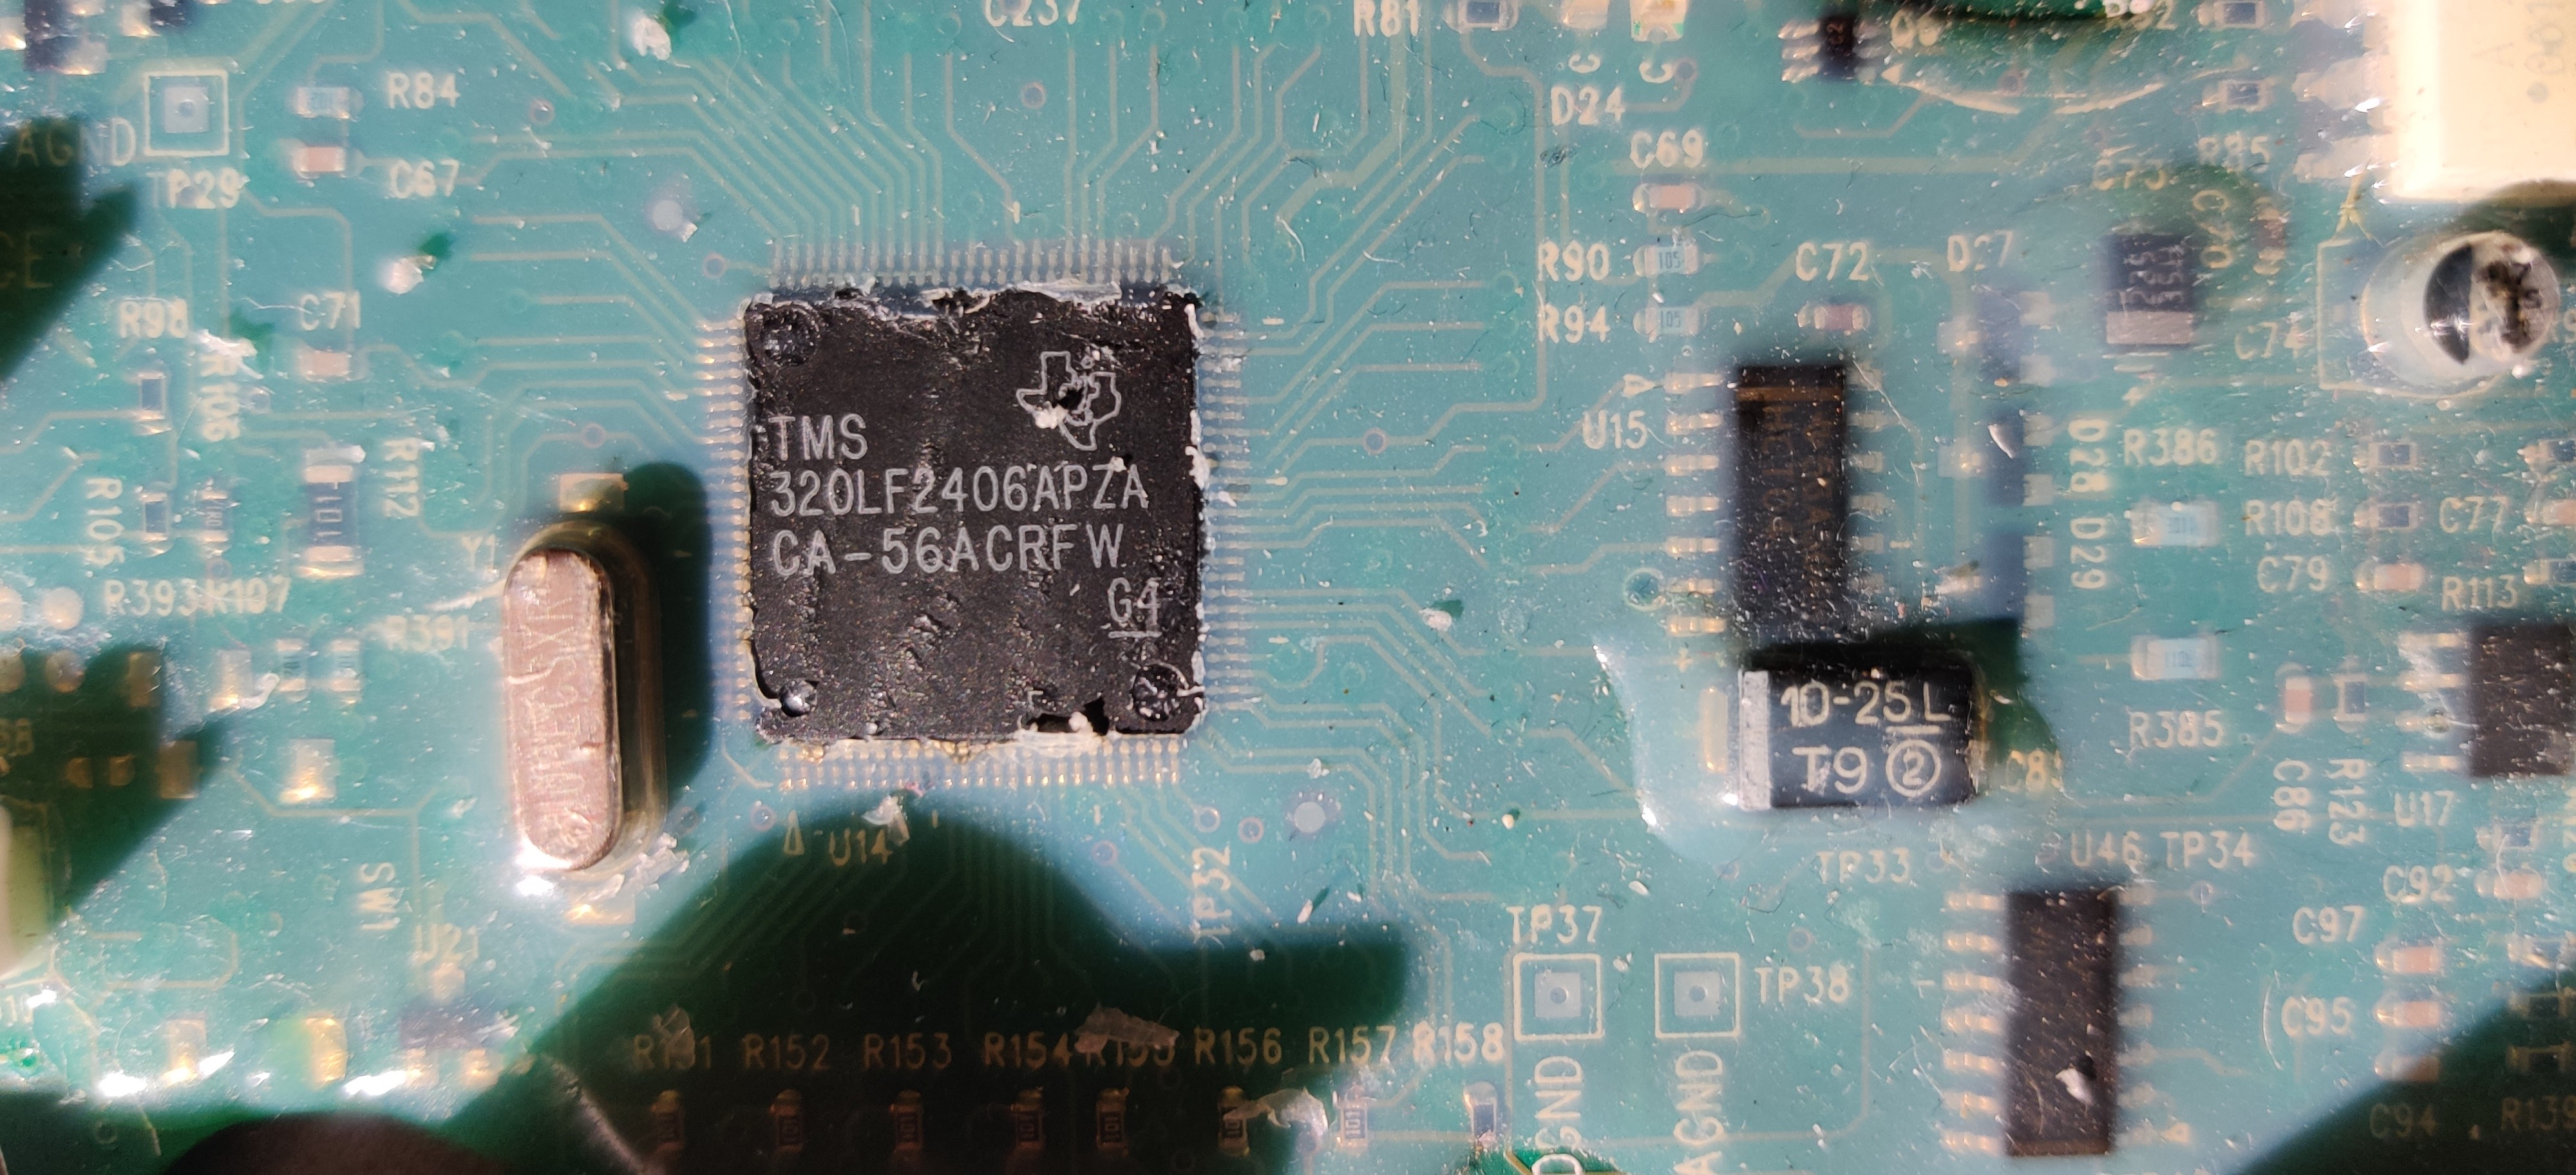
\includegraphics[]{chipImg-320LF2406APZA.jpg}
    \caption{caption}
    \label{fig:chipImg-320LF2406APZA.jpg}
\end{figure}

\begin{figure}
    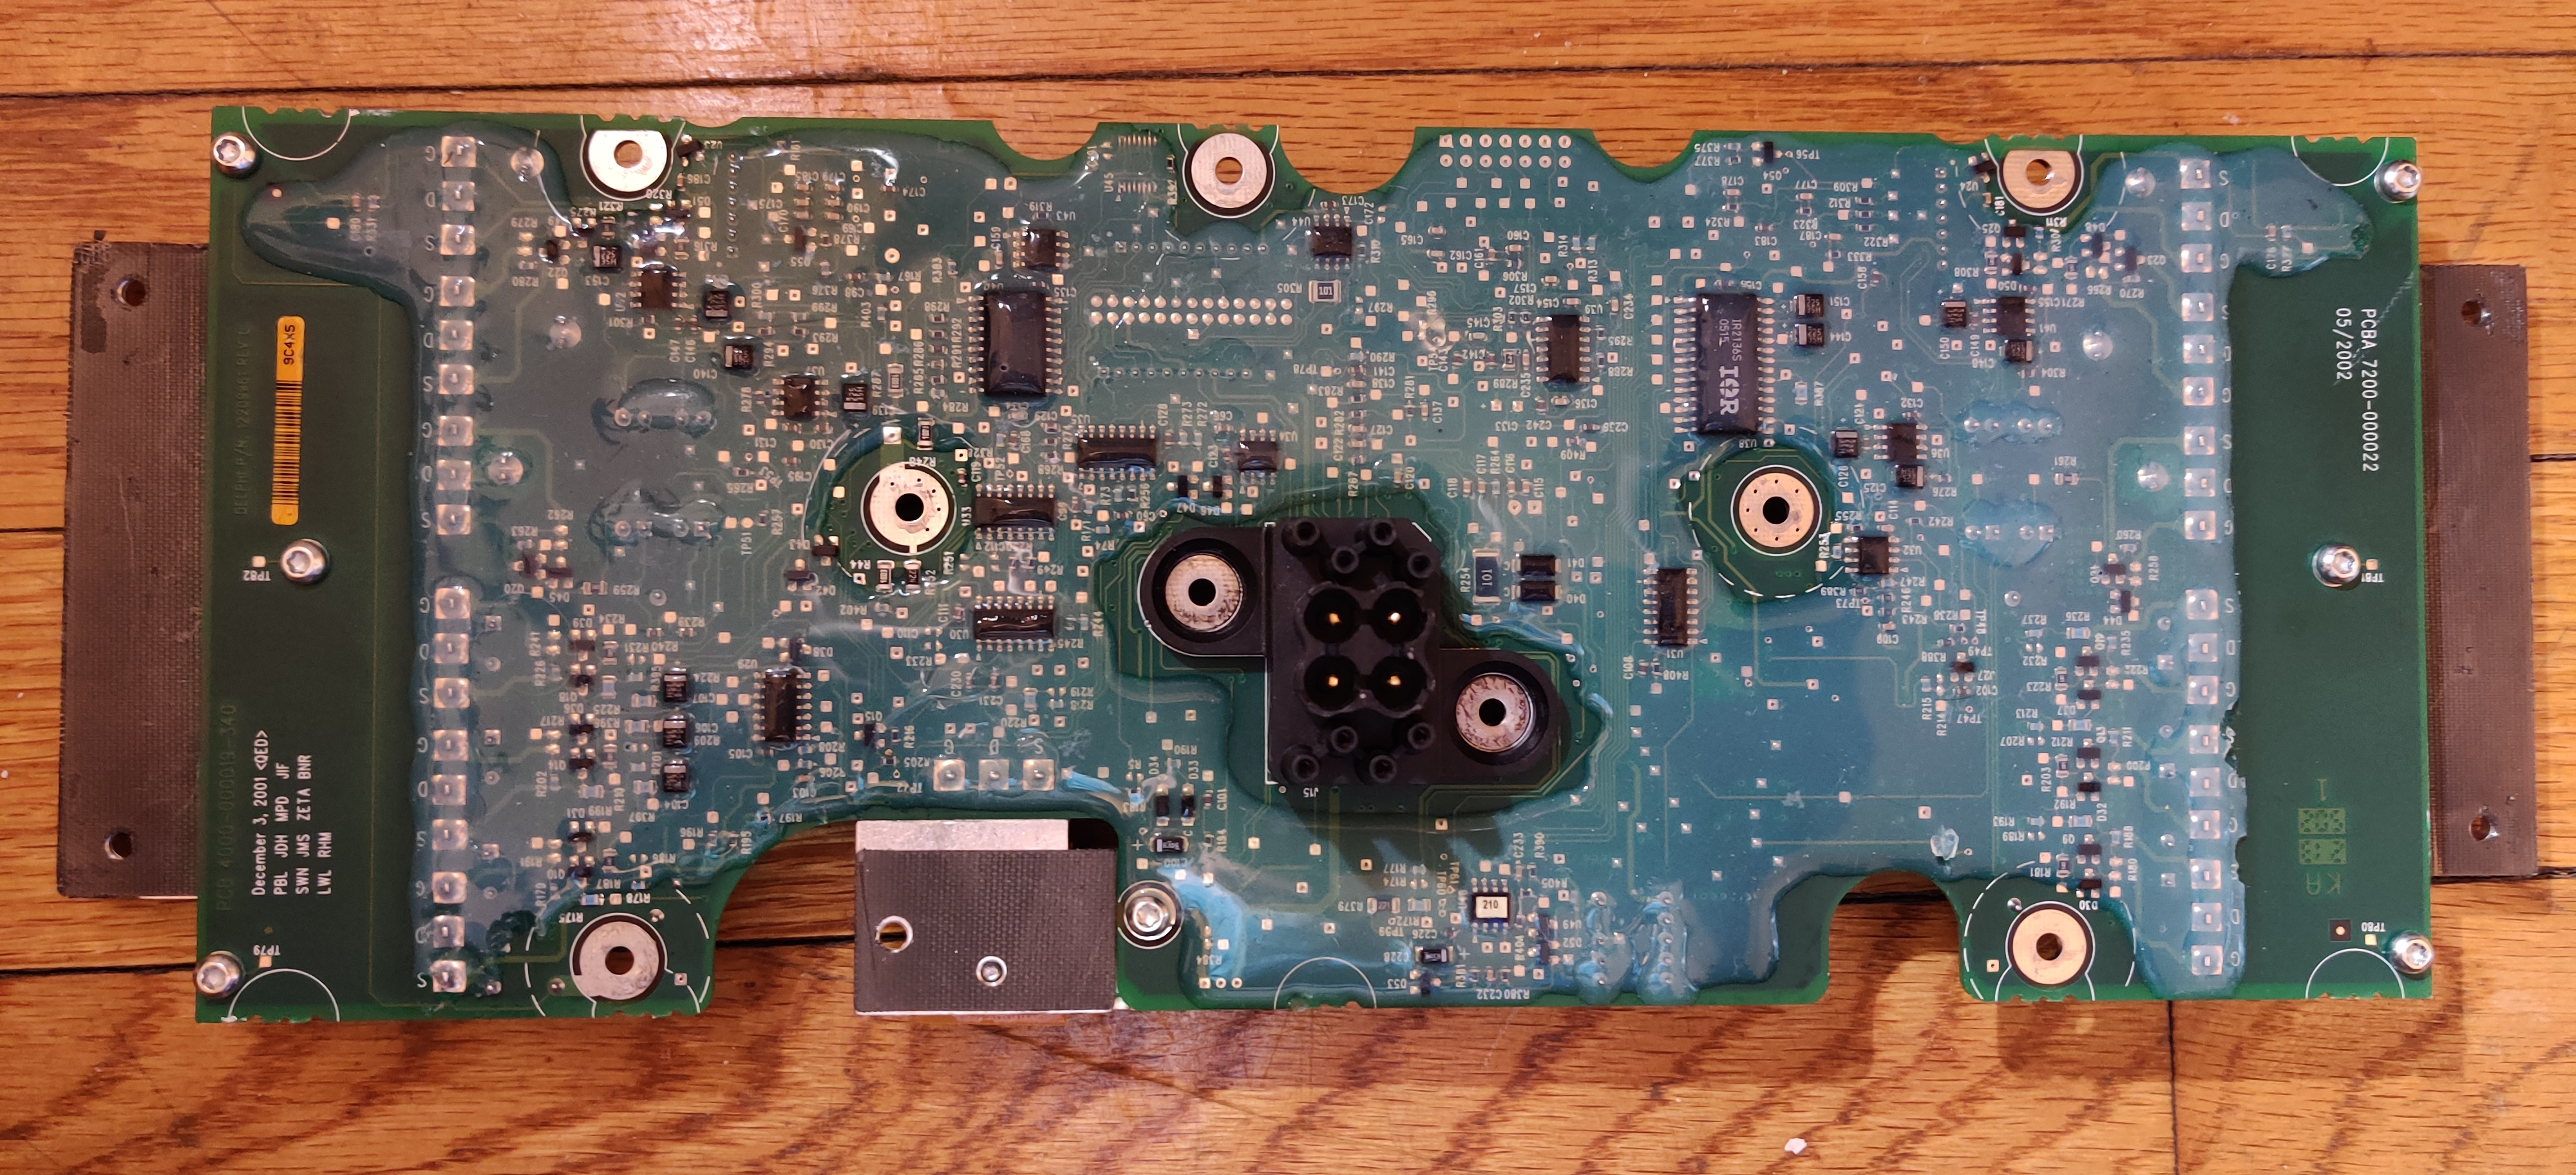
\includegraphics[]{entireBoardBottom.jpg}
    \caption{caption}
    \label{fig:entireBoardBottom.jpg}
\end{figure}

\begin{figure}
    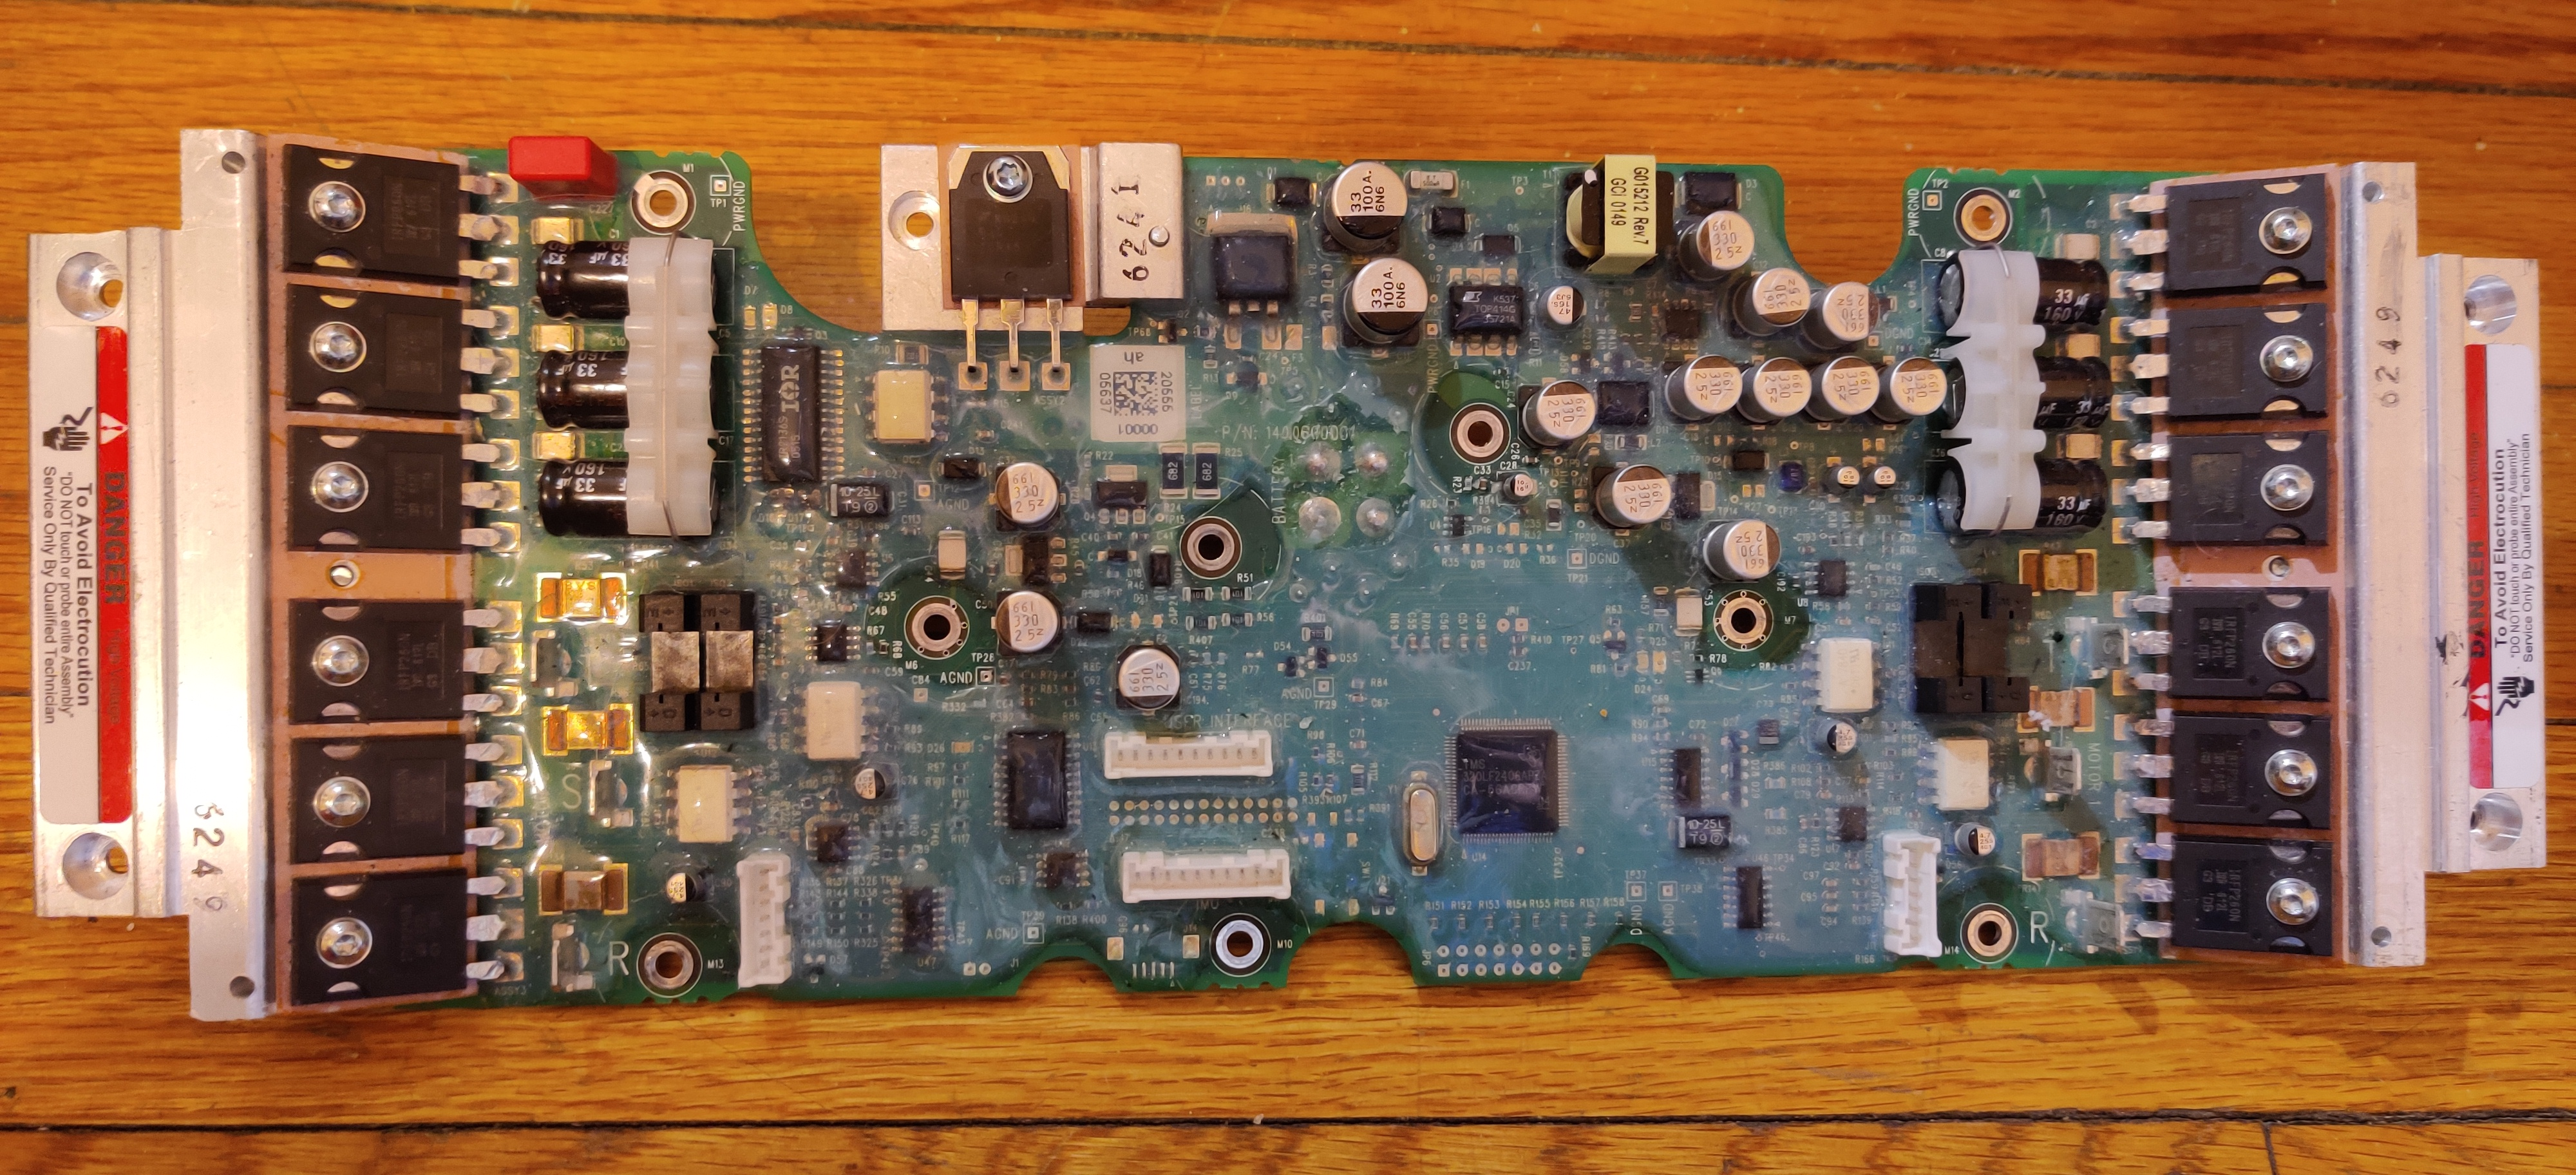
\includegraphics[]{entireBoardTop.jpg}
    \caption{caption}
    \label{fig:entireBoardTop.jpg}
\end{figure}

\begin{figure}
    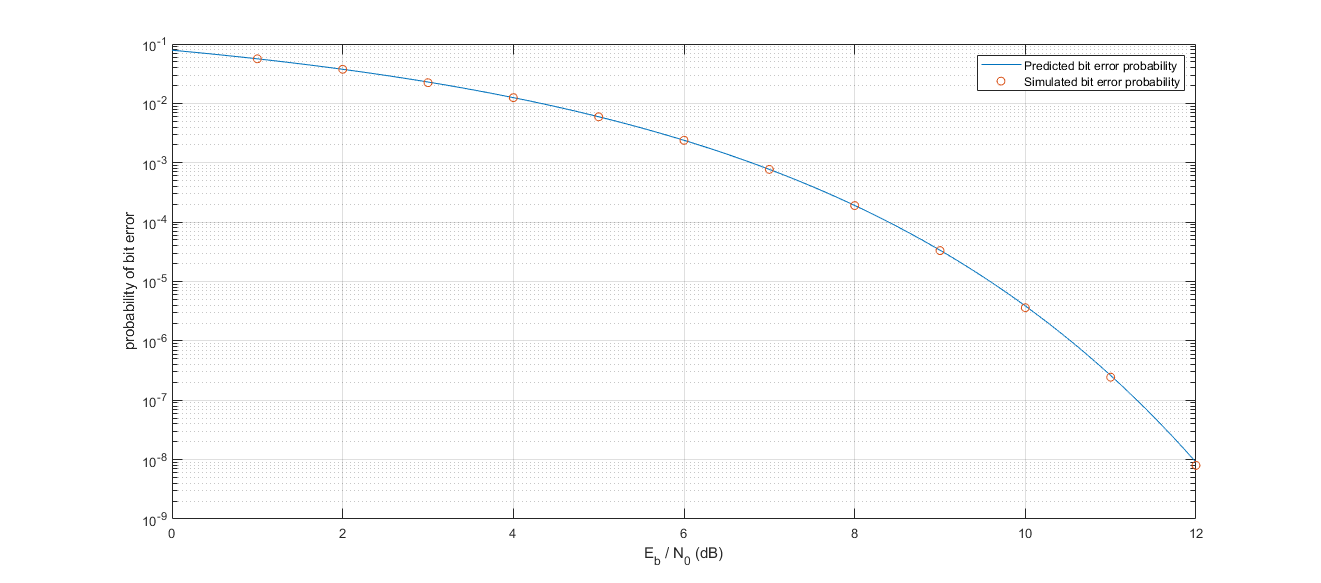
\includegraphics[]{report.png}
    \caption{caption}
    \label{fig:report.png} 
\end{figure}

\begin{figure}
    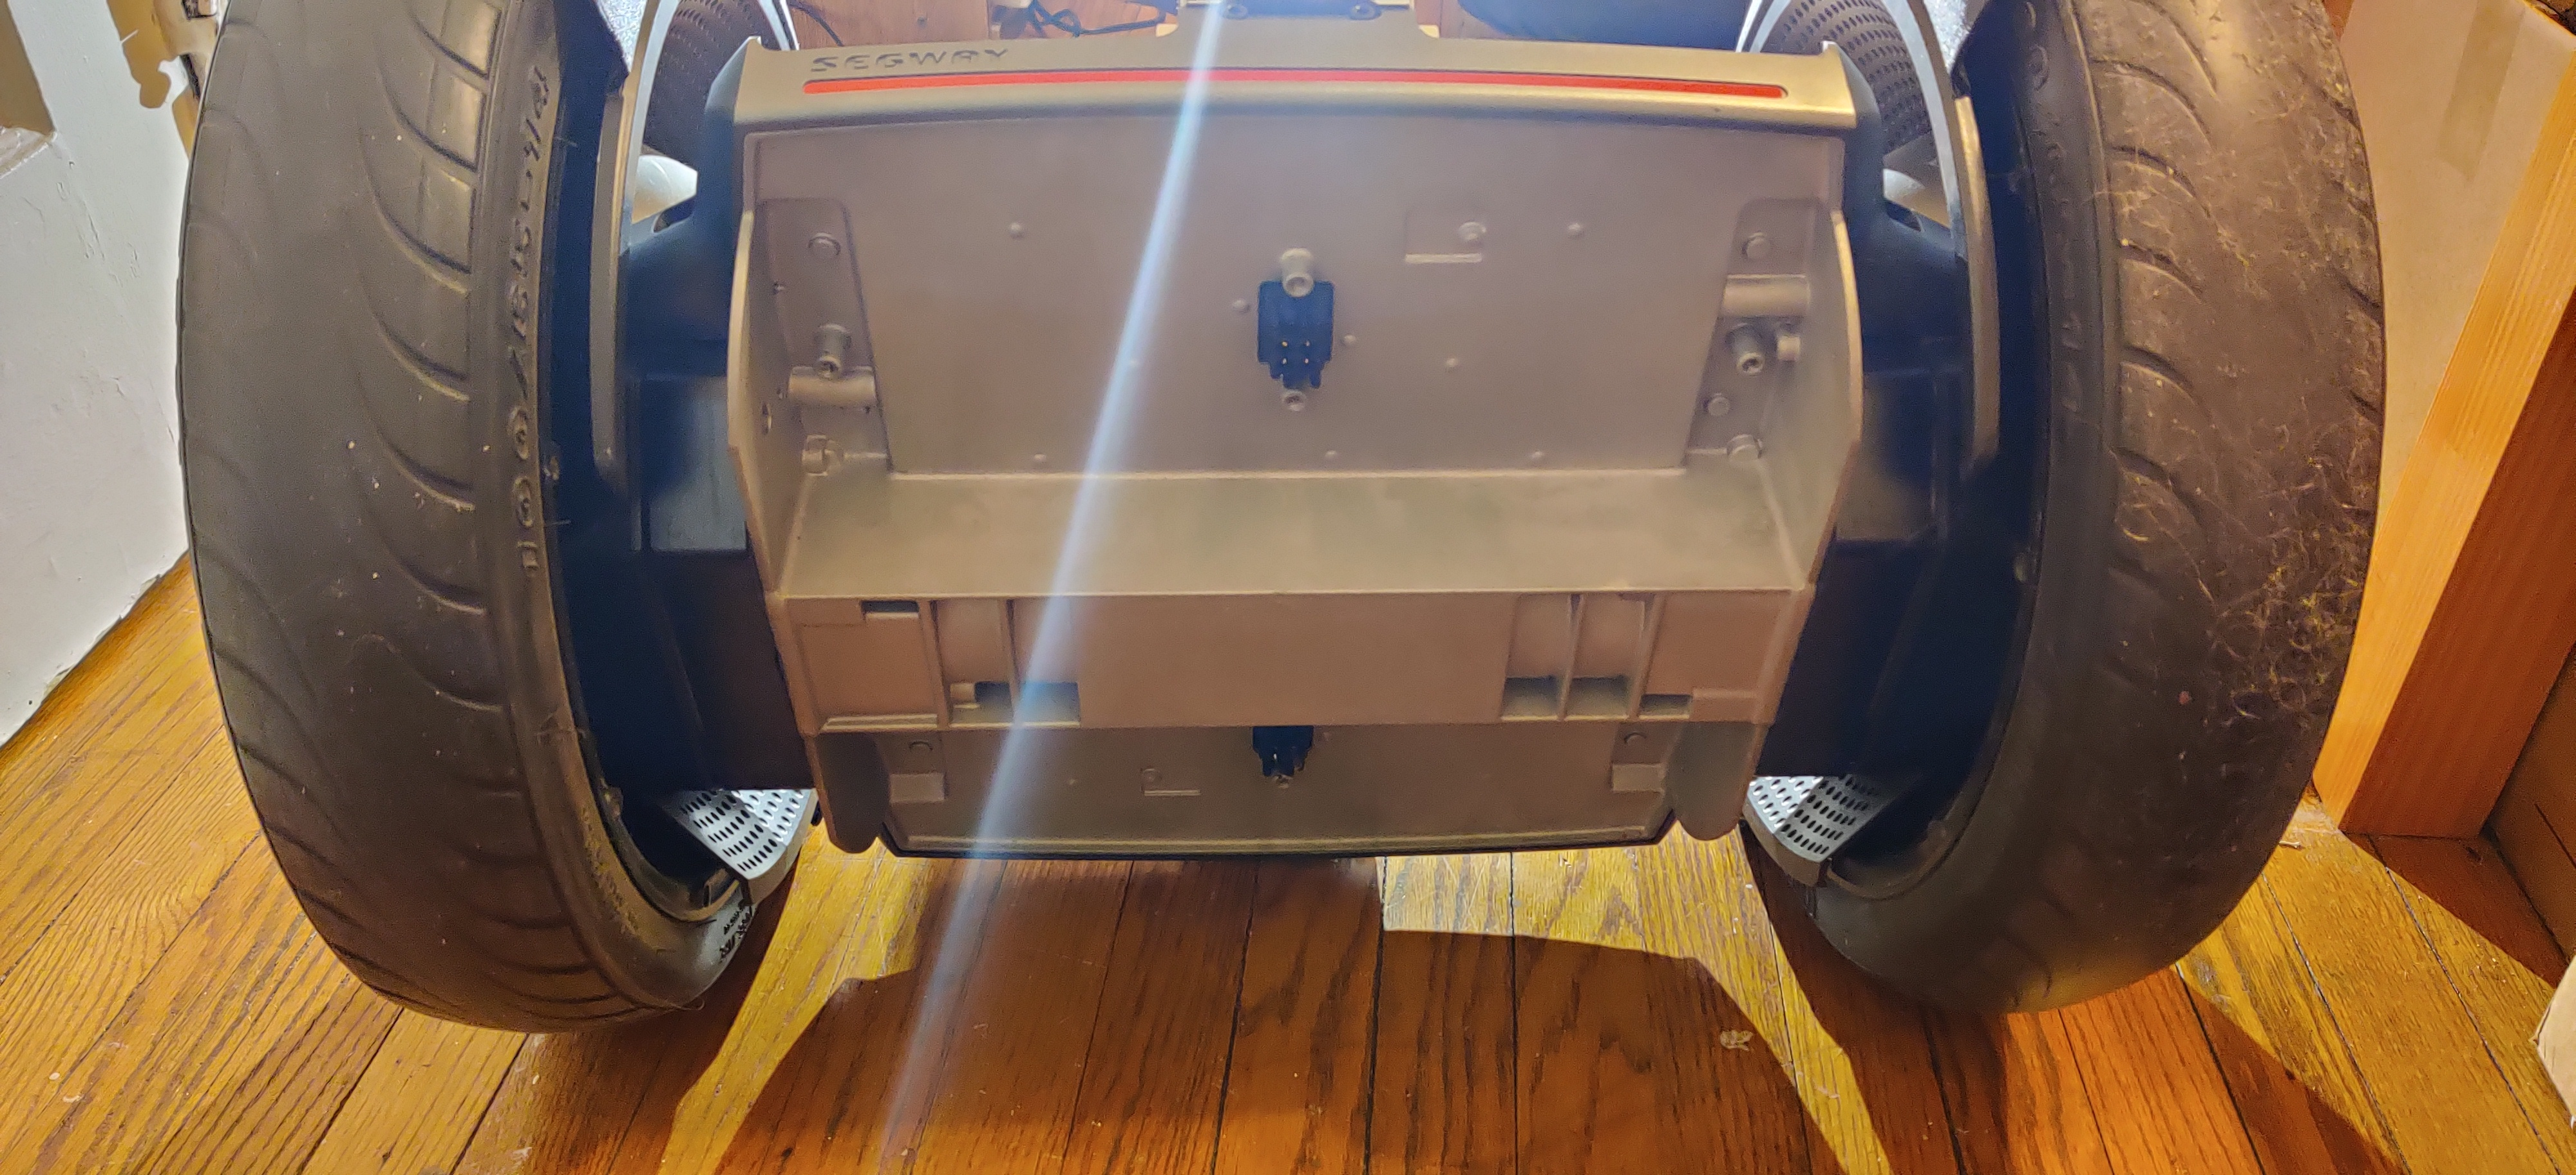
\includegraphics[]{segwayBottom.jpg}
    \caption{caption}
    \label{fig:segwayBottom.jpg}
\end{figure}

\begin{figure}
    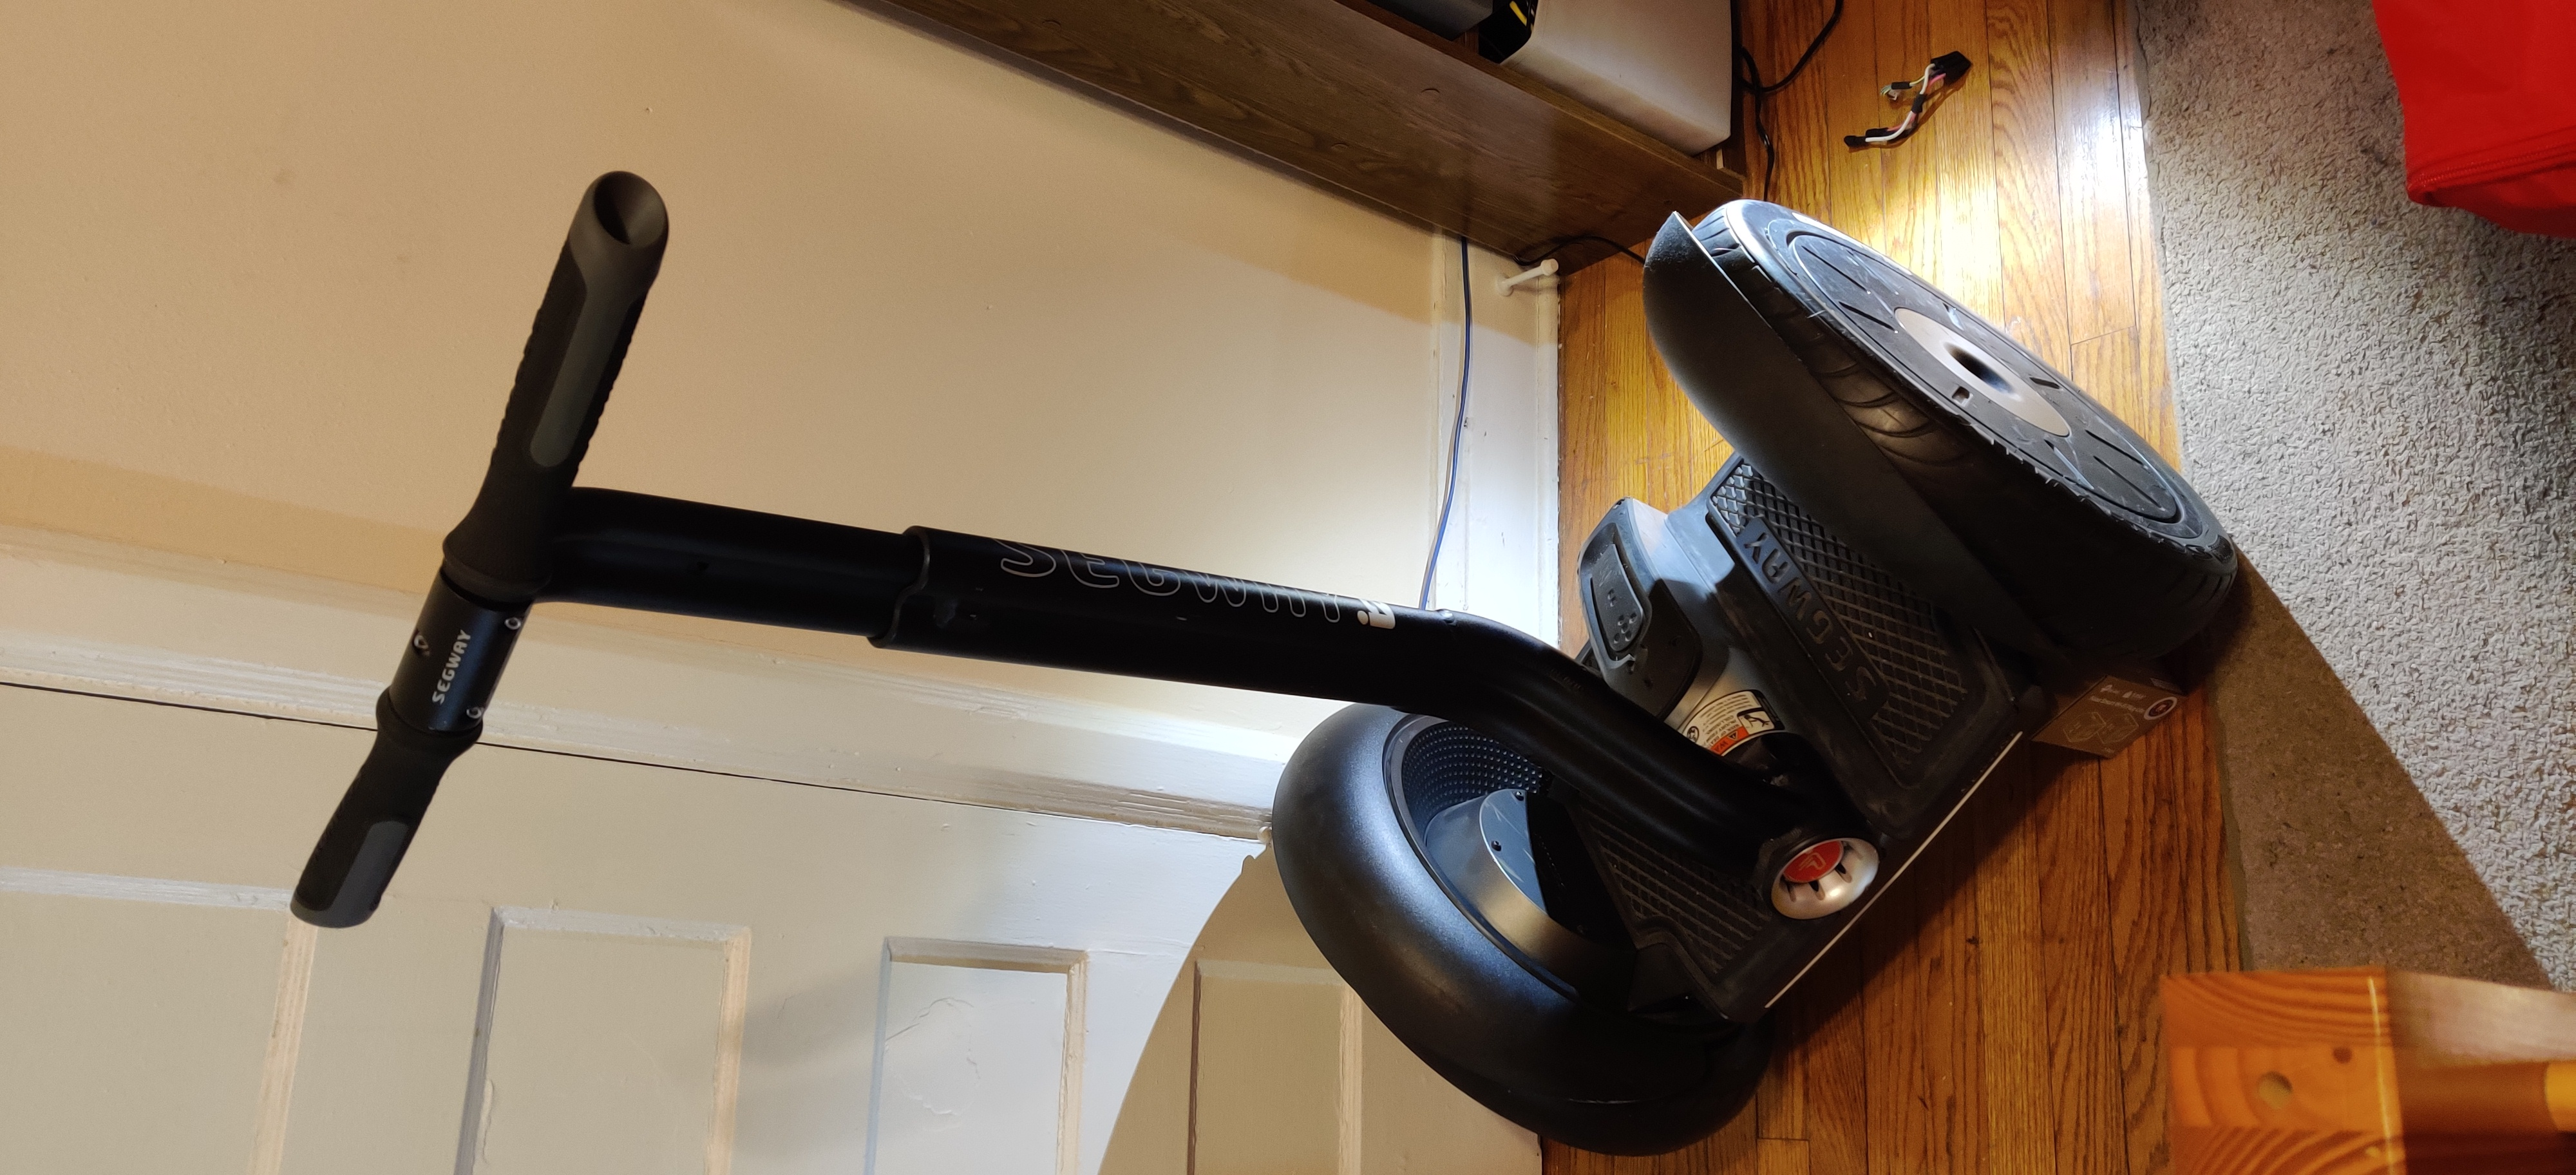
\includegraphics[]{segwayFront.jpg}
    \caption{caption}
    \label{fig:segwayFront.jpg}
\end{figure}

\begin{figure}
    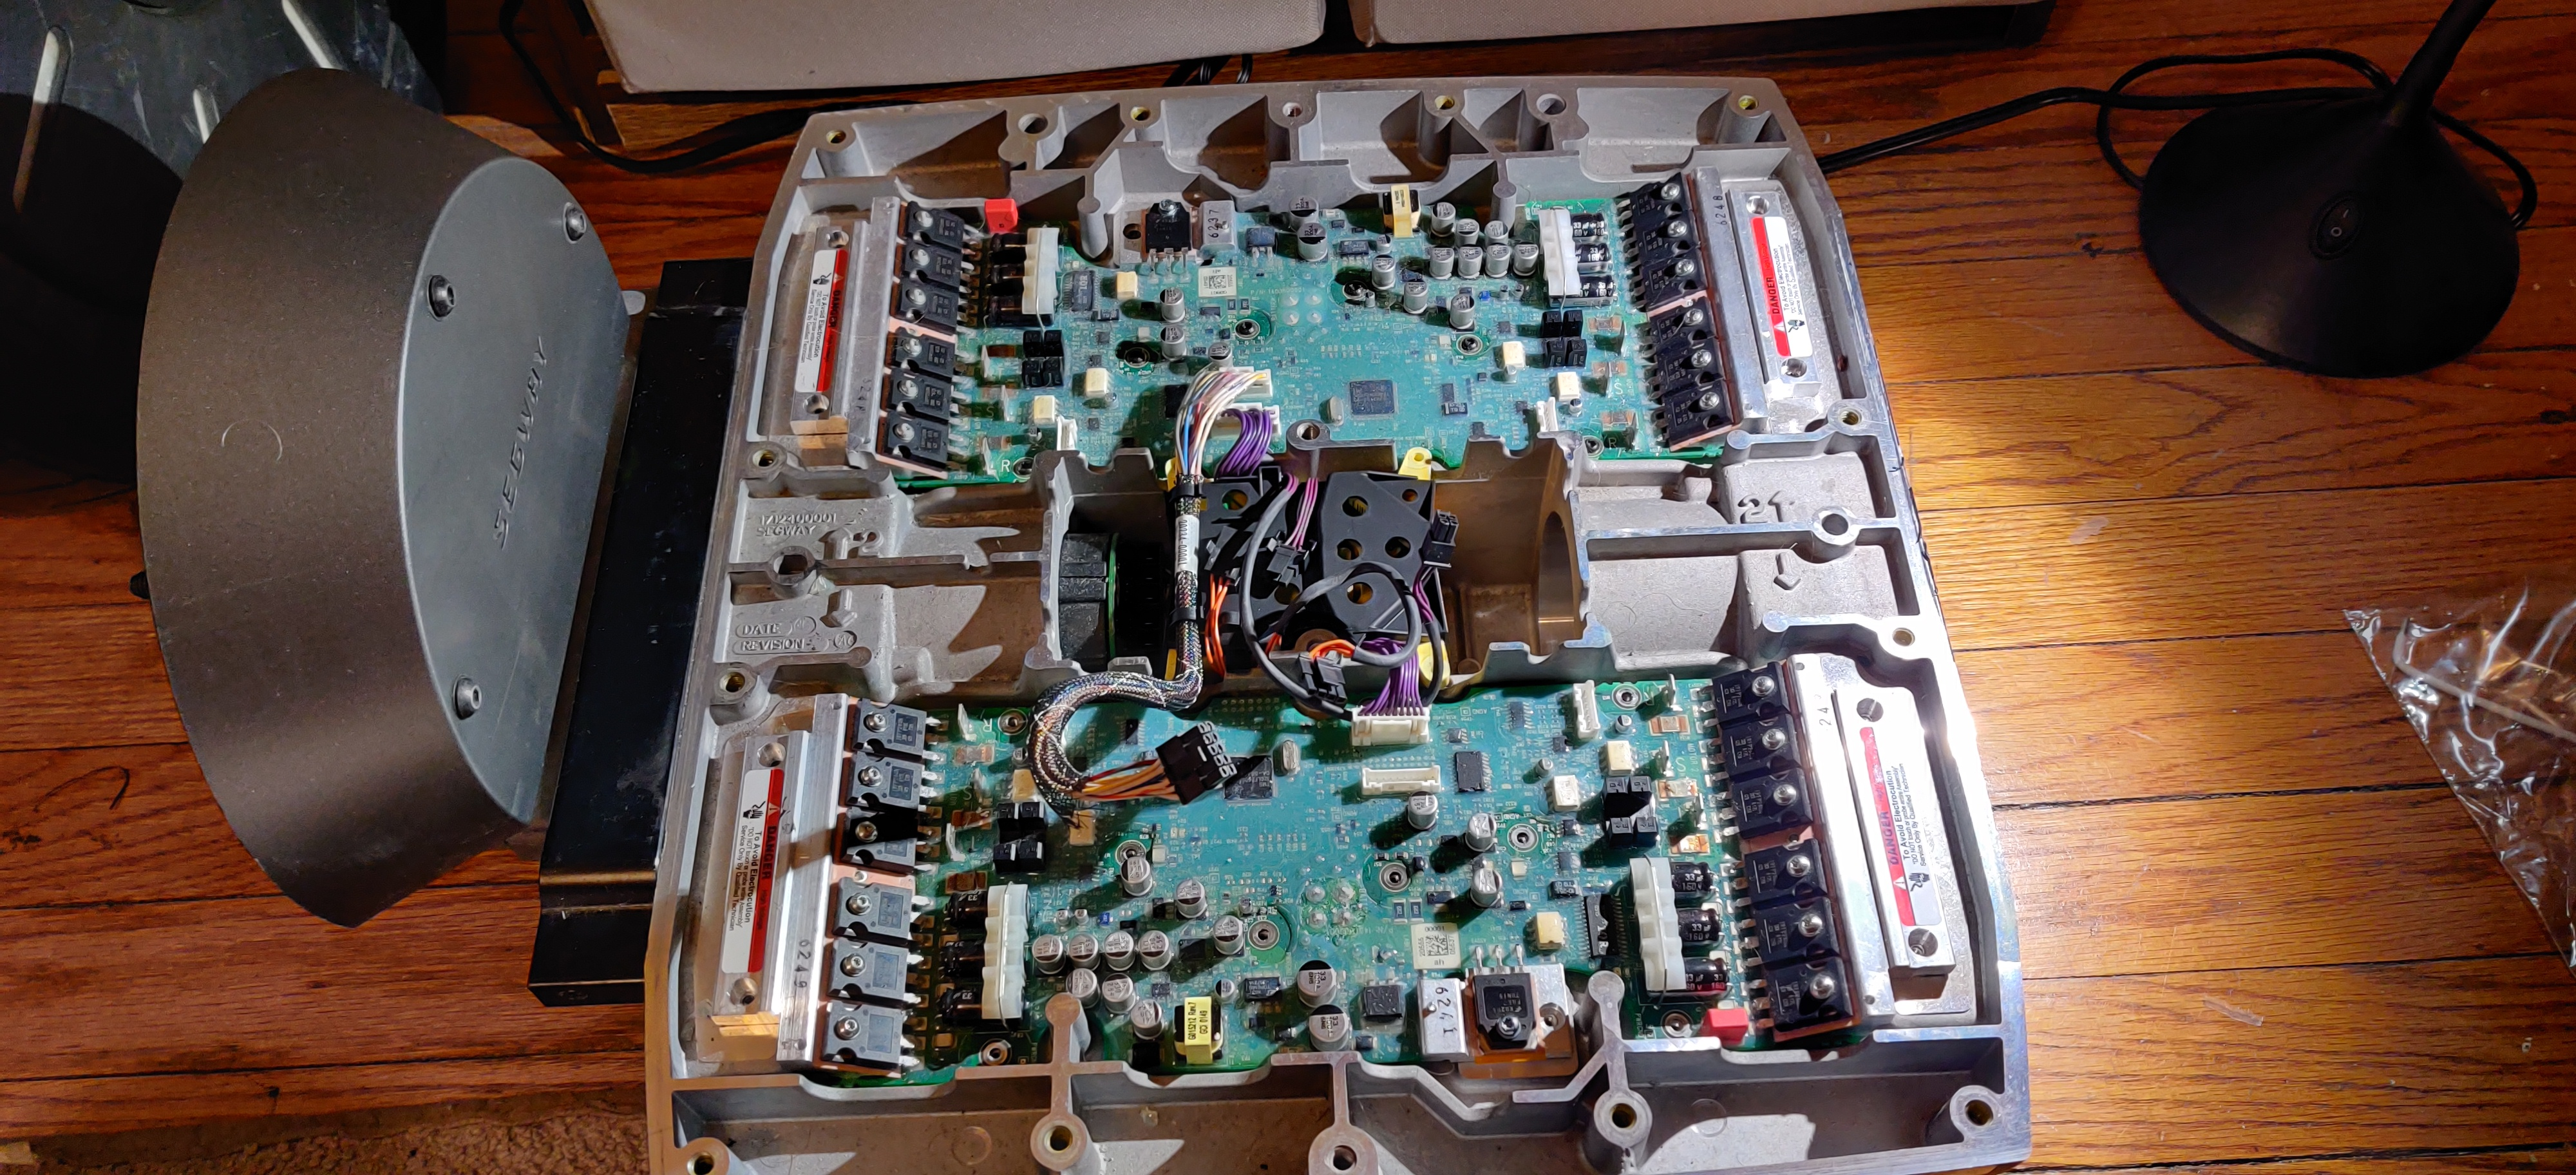
\includegraphics[]{segwayInternalsTop.jpg}
    \caption{caption}
    \label{fig:segwayInternalsTop.jpg}
\end{figure}

\begin{figure}
    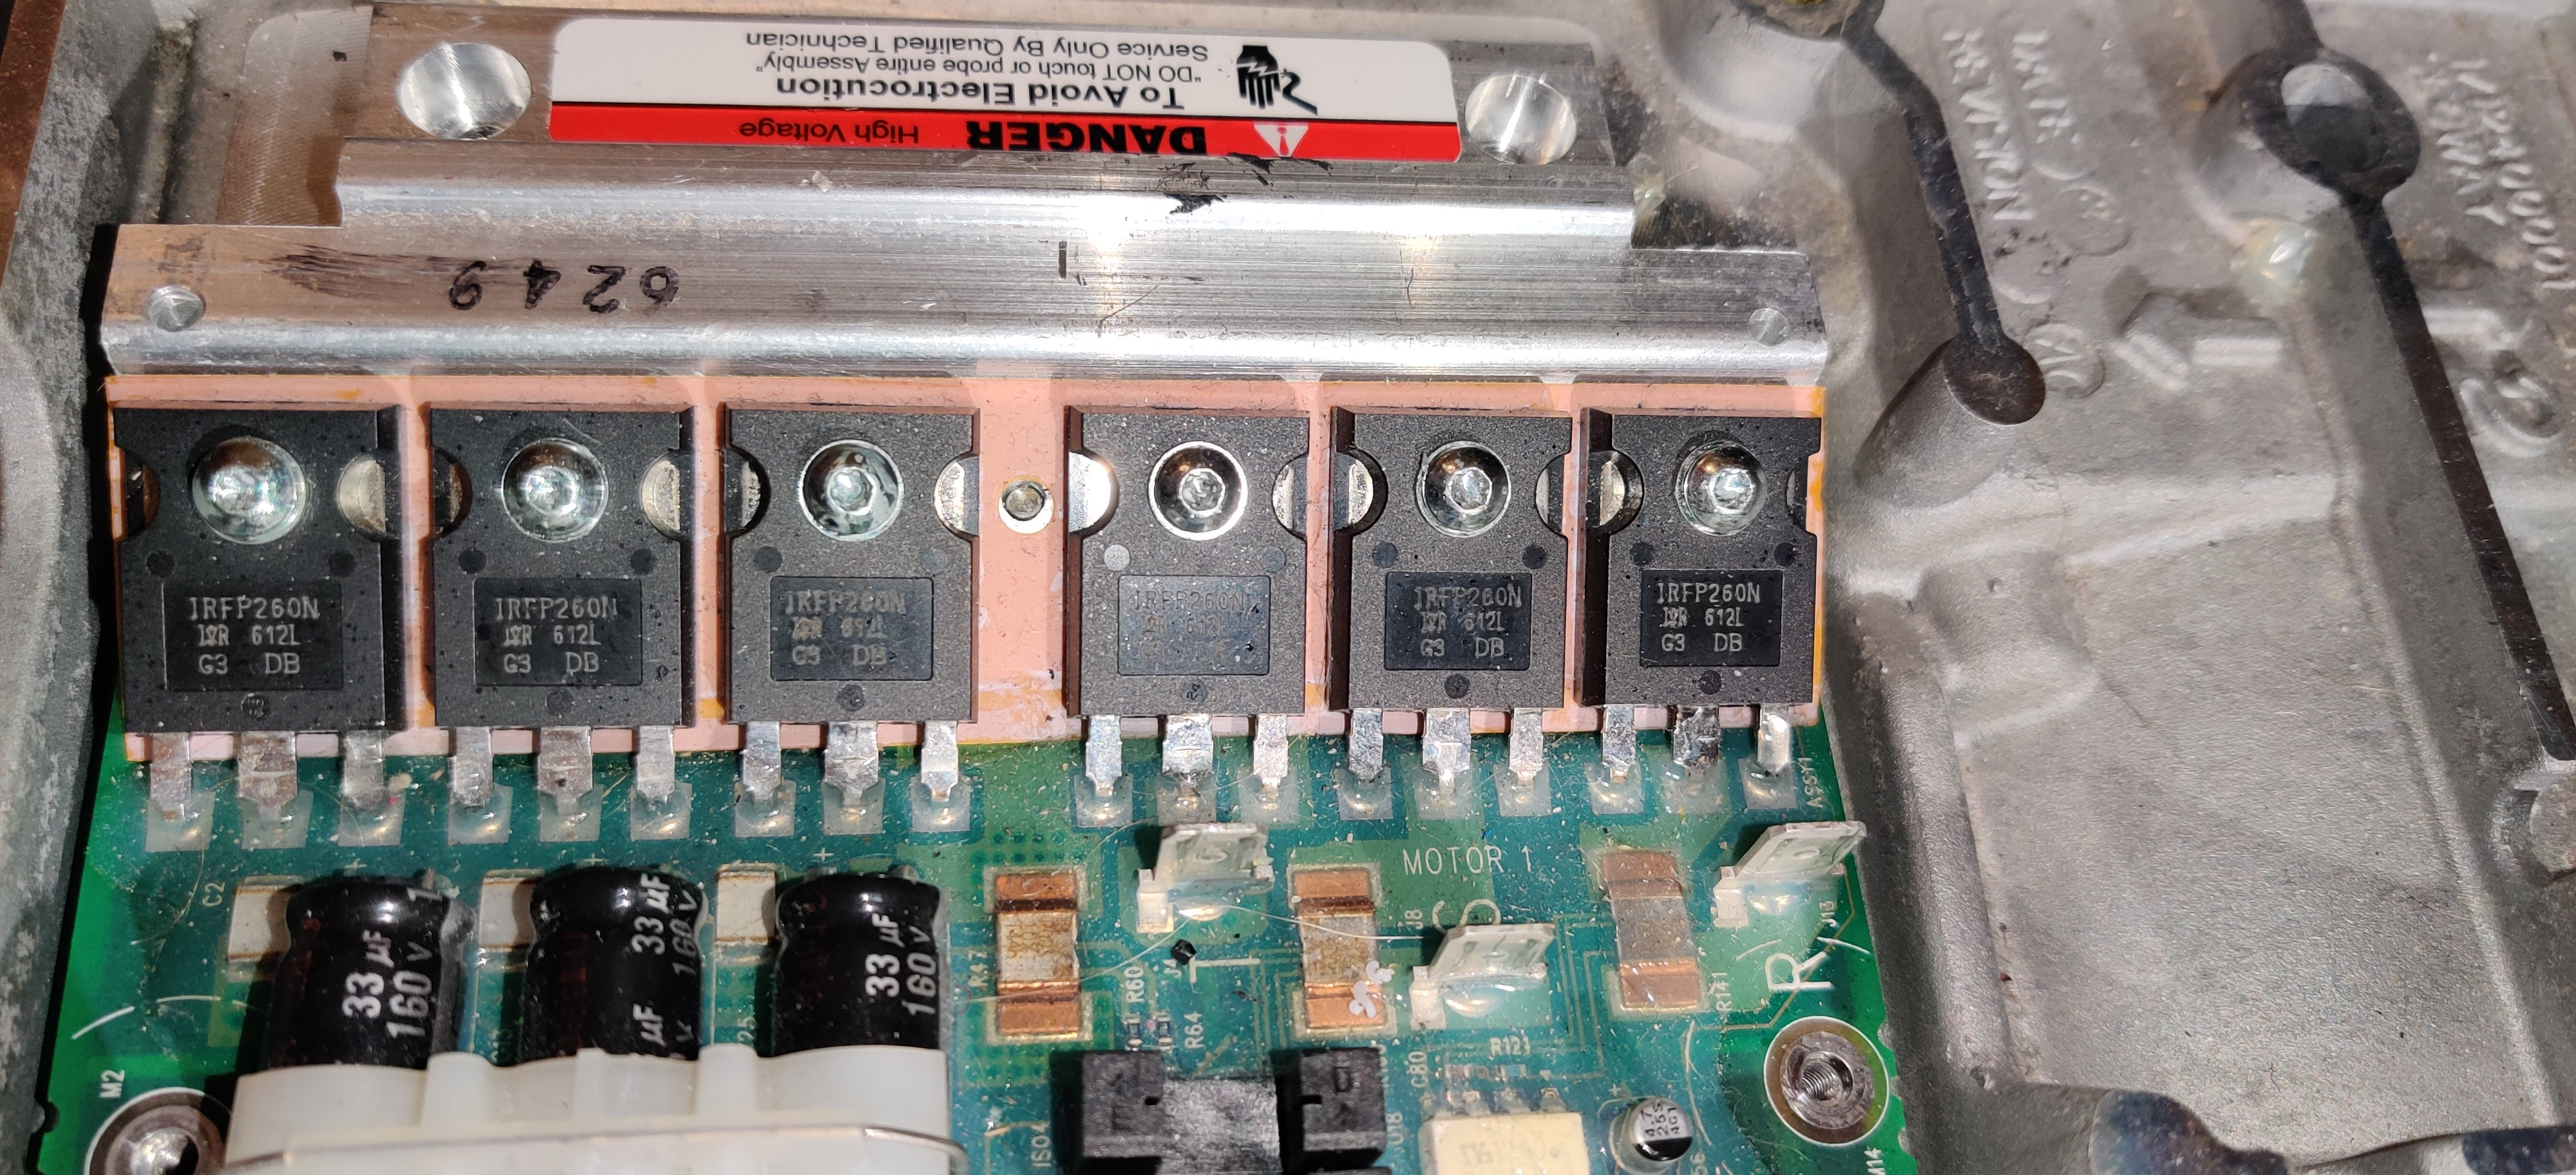
\includegraphics[]{segwayMotorDrivers.jpg}
    \caption{caption}
    \label{fig:segwayMotorDrivers.jpg}
\end{figure}

\begin{figure}
    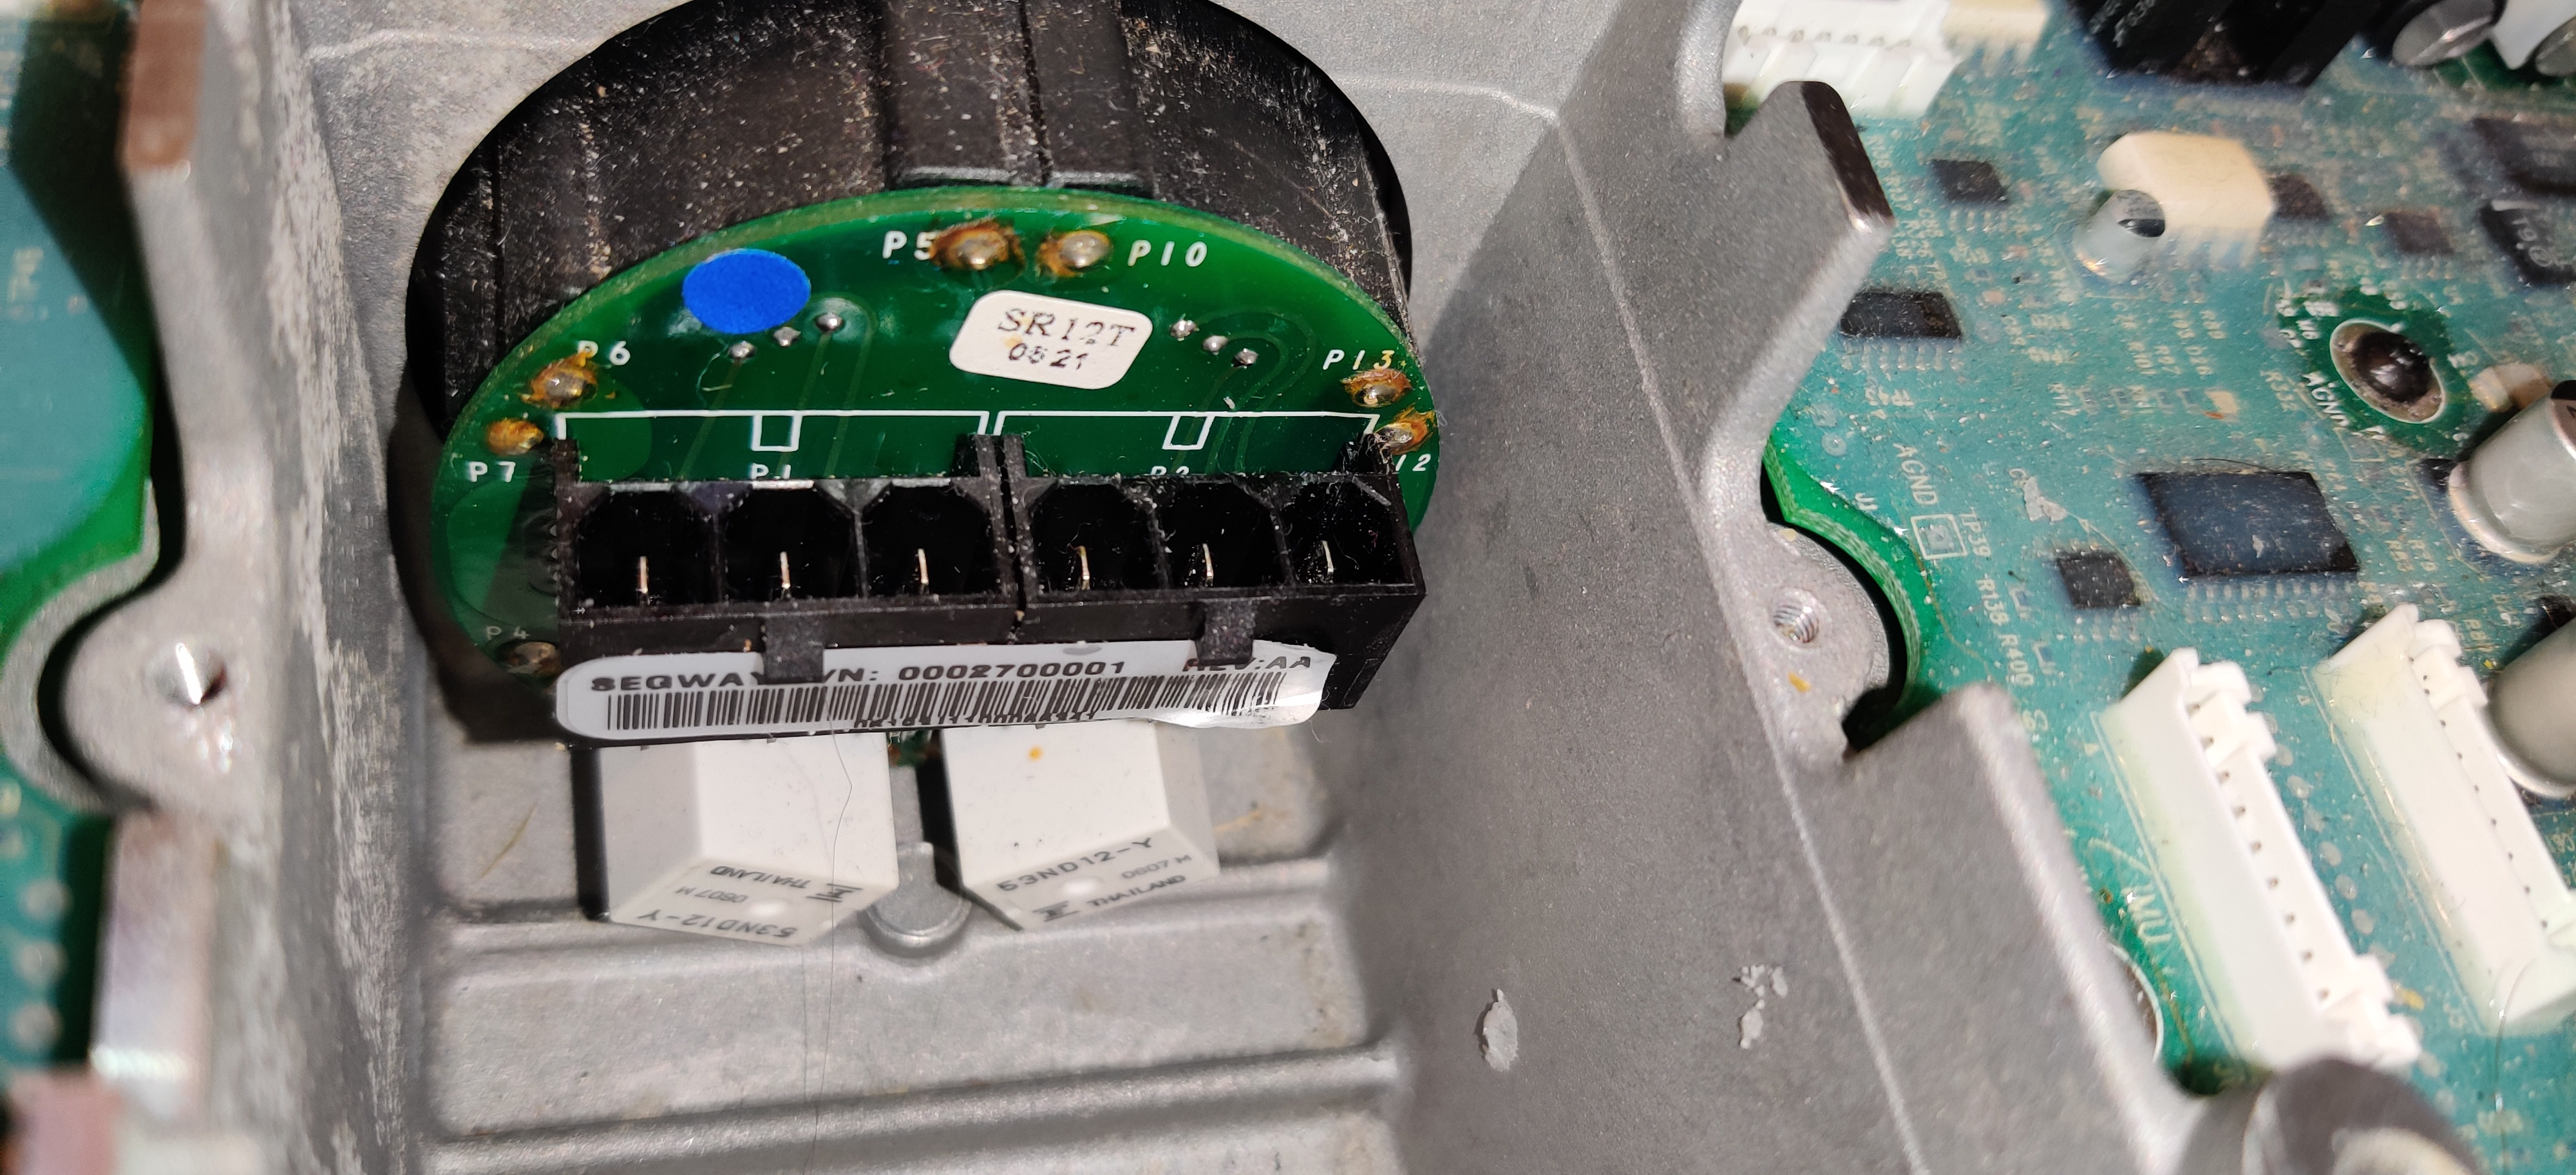
\includegraphics[]{segwayMotorInternal.jpg}
    \caption{caption}
    \label{fig:segwayMotorInternal.jpg}
\end{figure}

\begin{figure}
    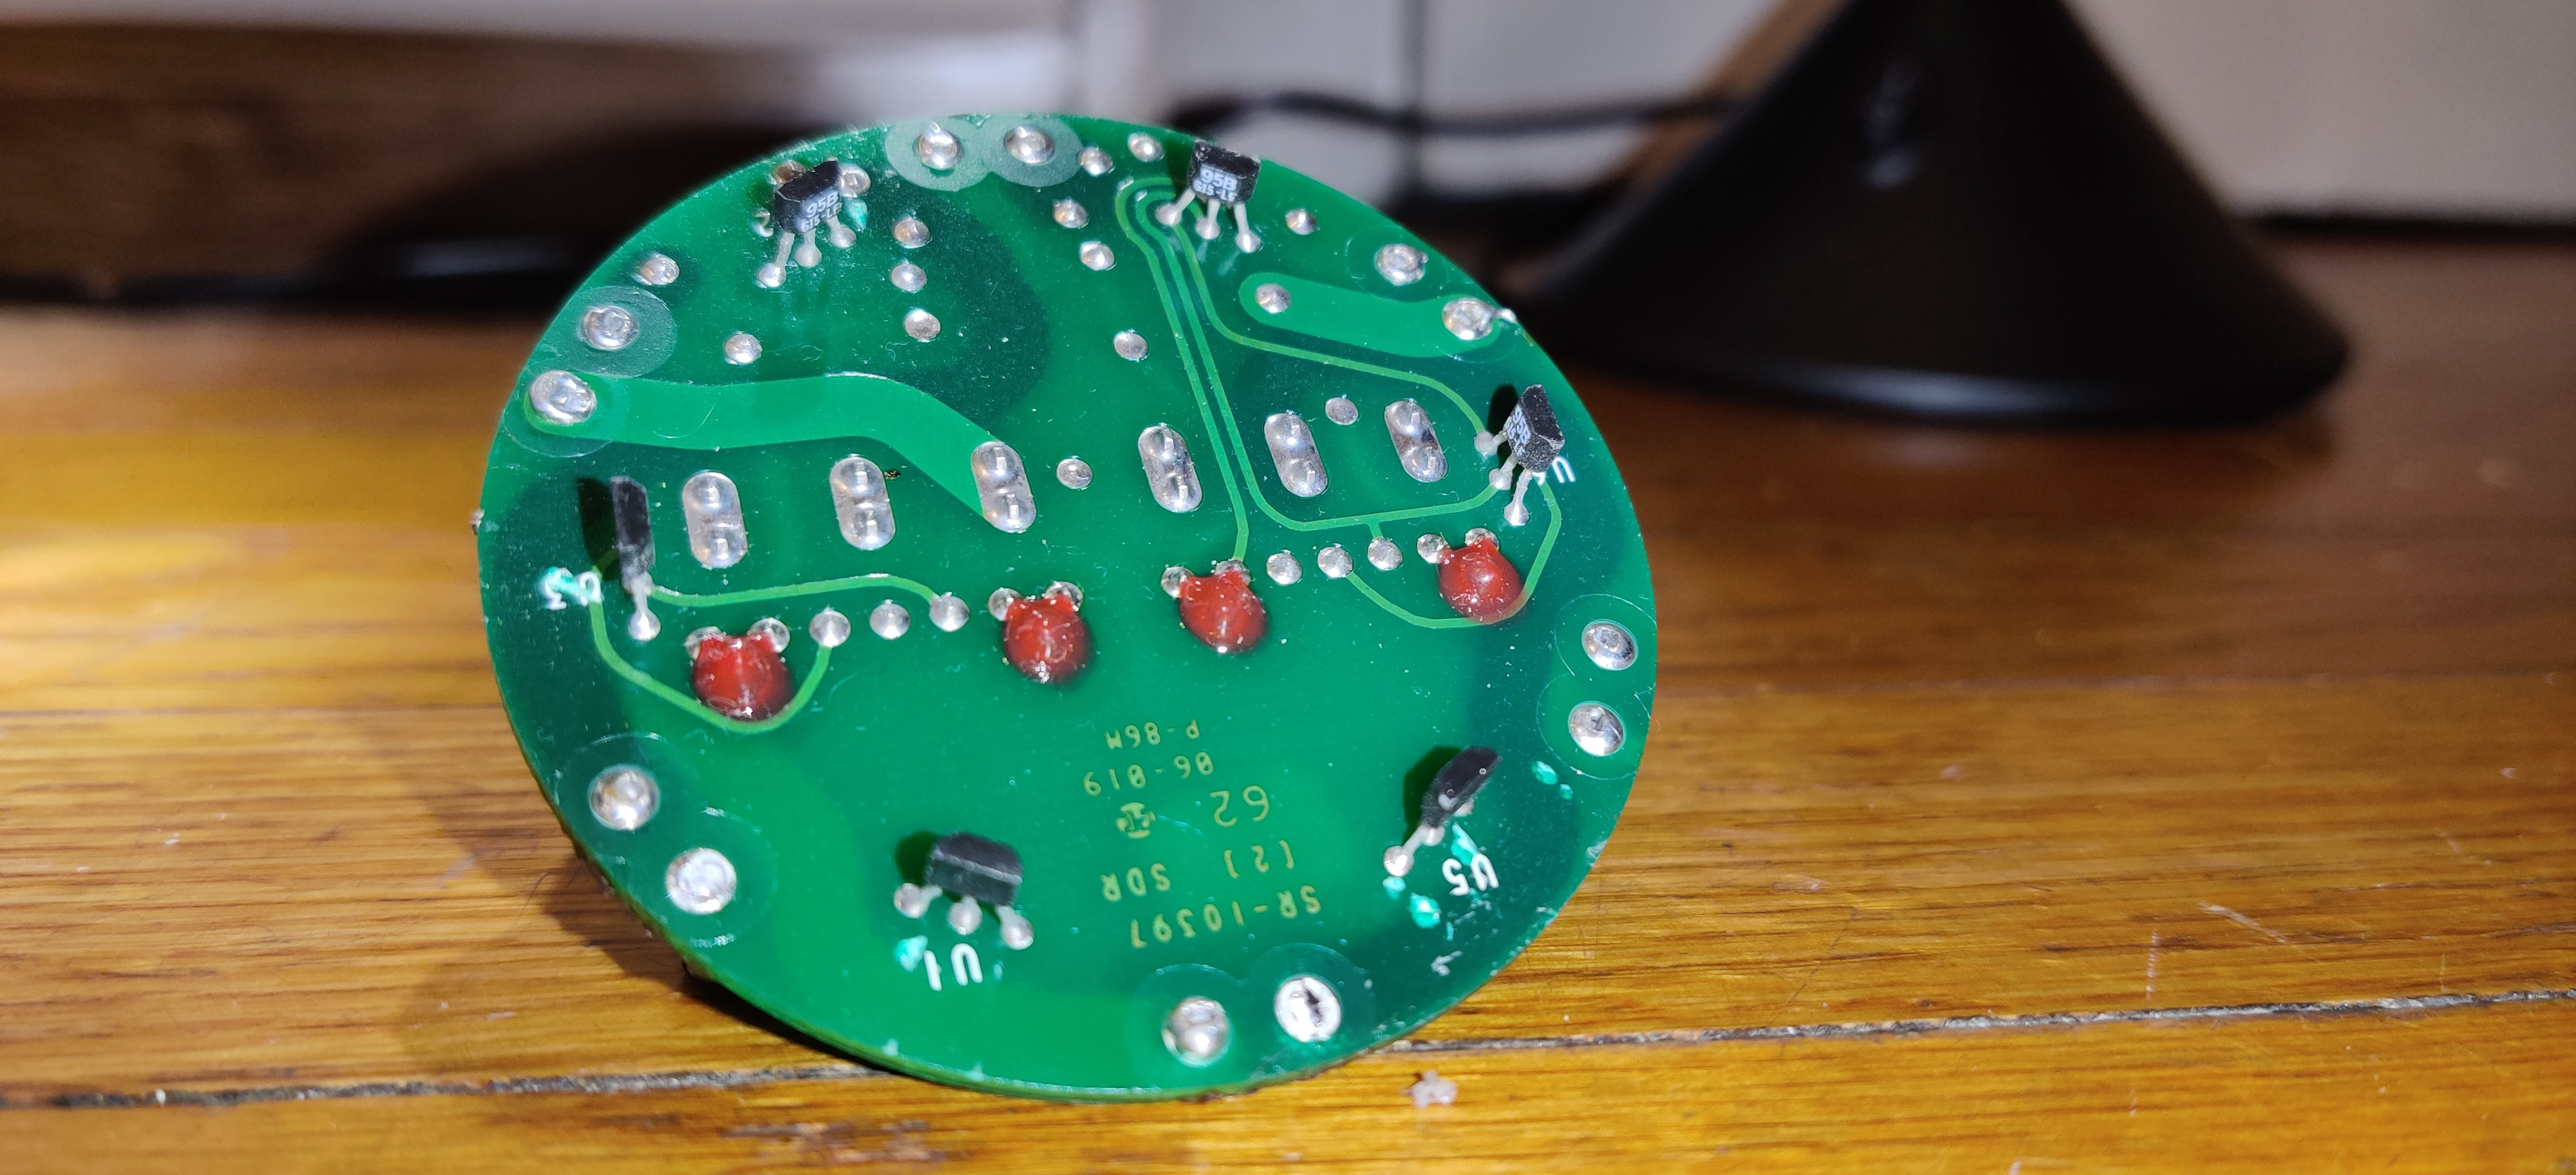
\includegraphics[]{segwayMotorPCBRear.jpg}
    \caption{caption}
    \label{fig:segwayMotorPCBRear.jpg}
\end{figure}

\begin{figure}
    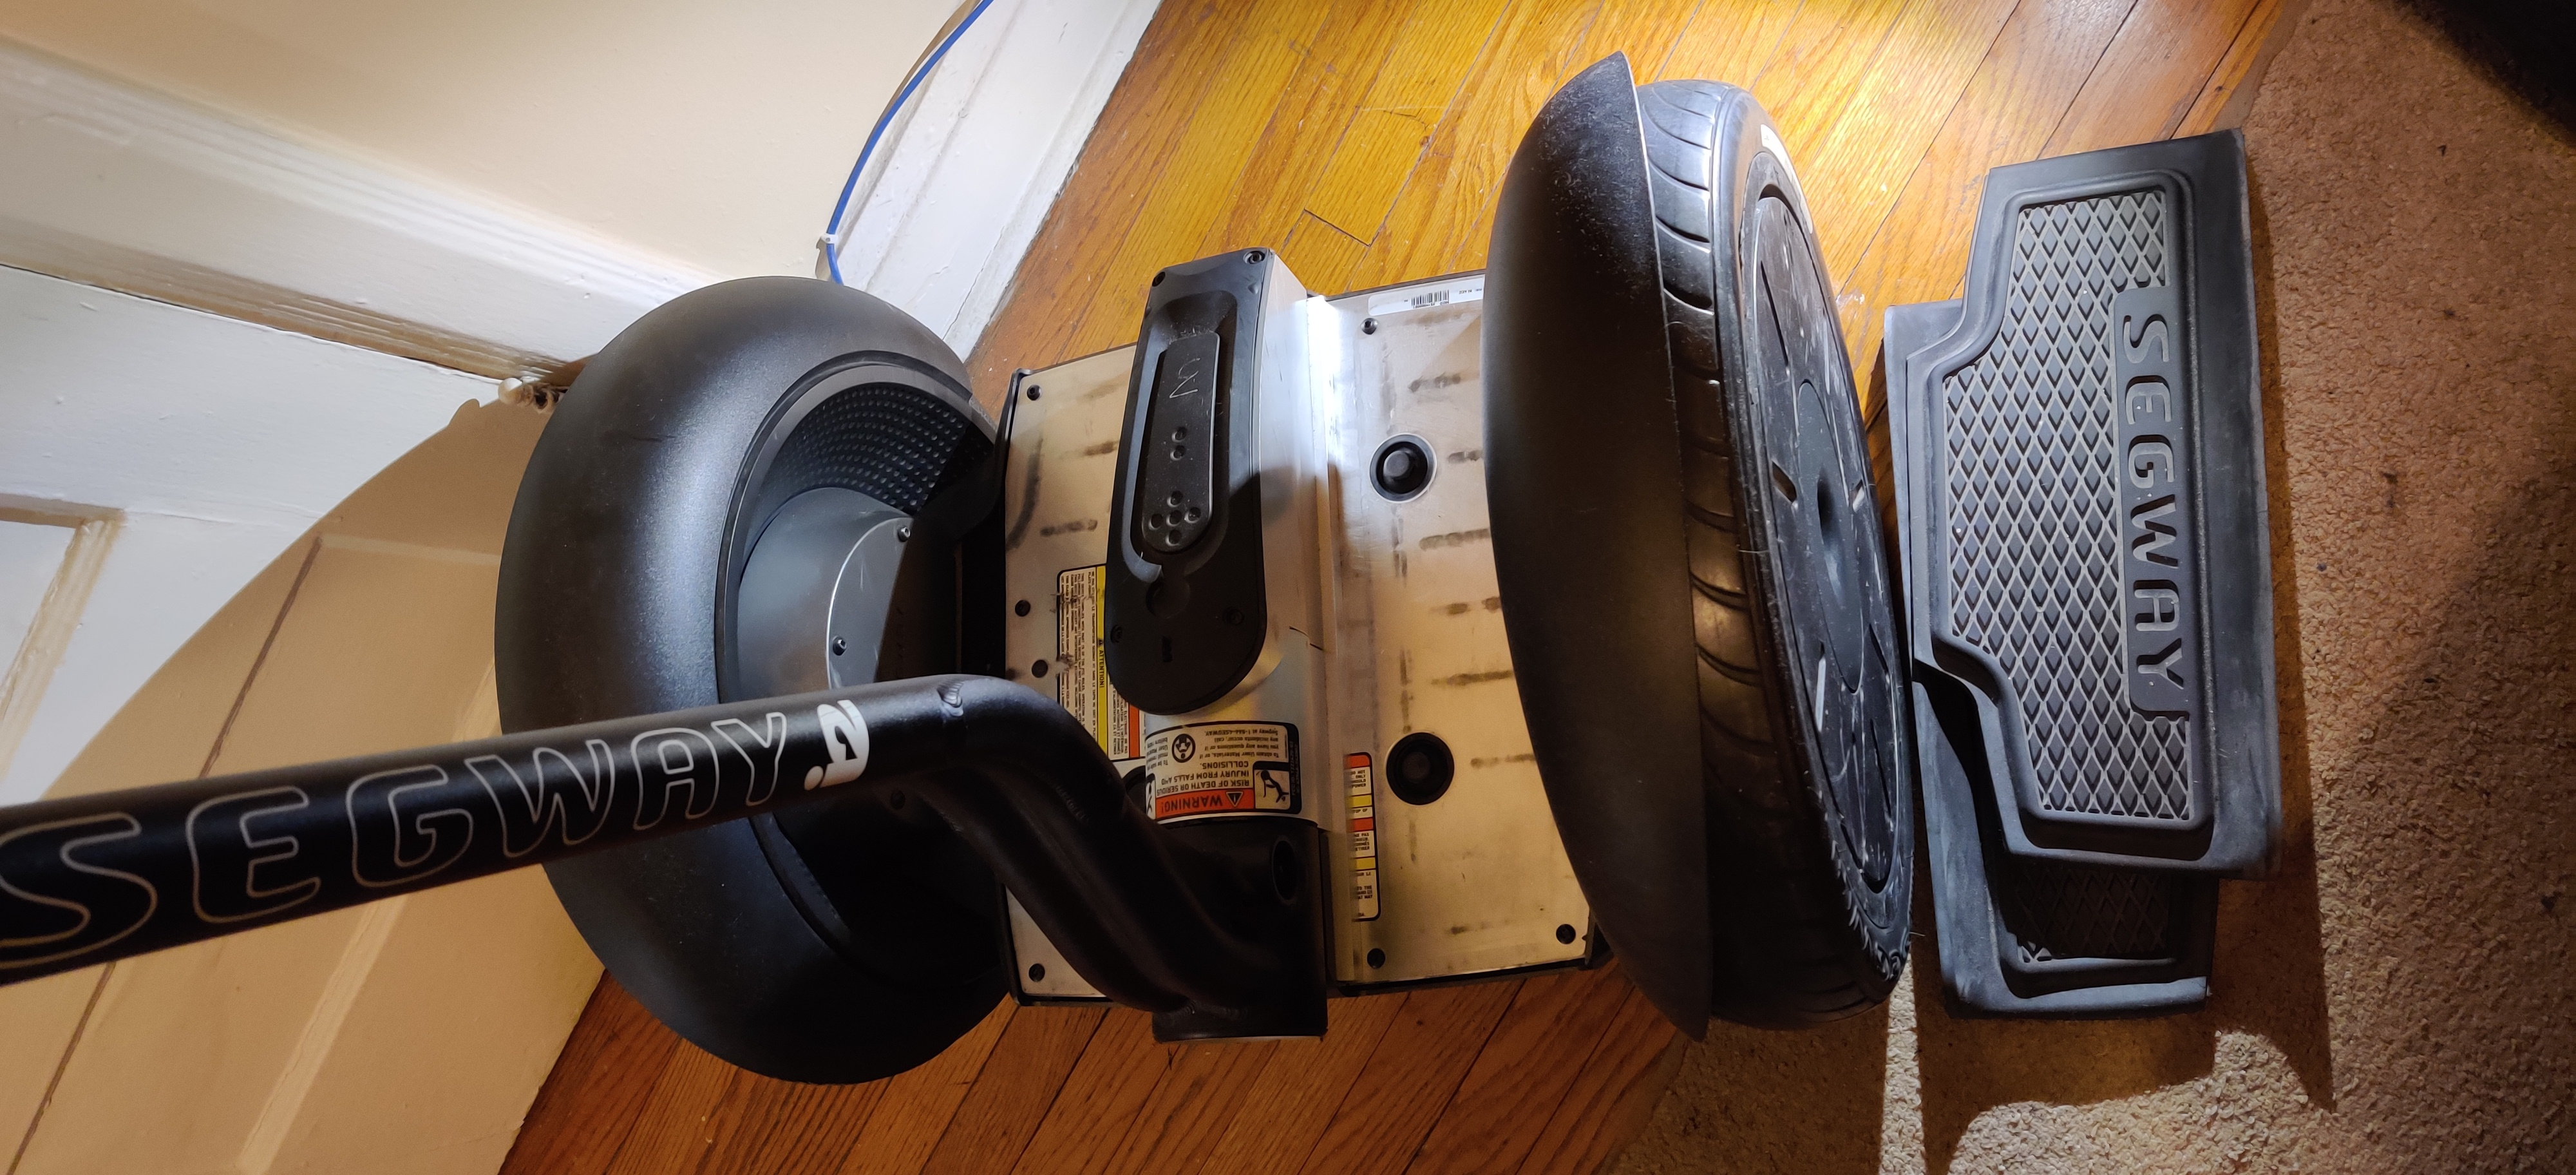
\includegraphics[]{segwayPadsRemoved.jpg}
    \caption{caption}
    \label{fig:segwayPadsRemoved.jpg}
\end{figure}

\begin{figure}
    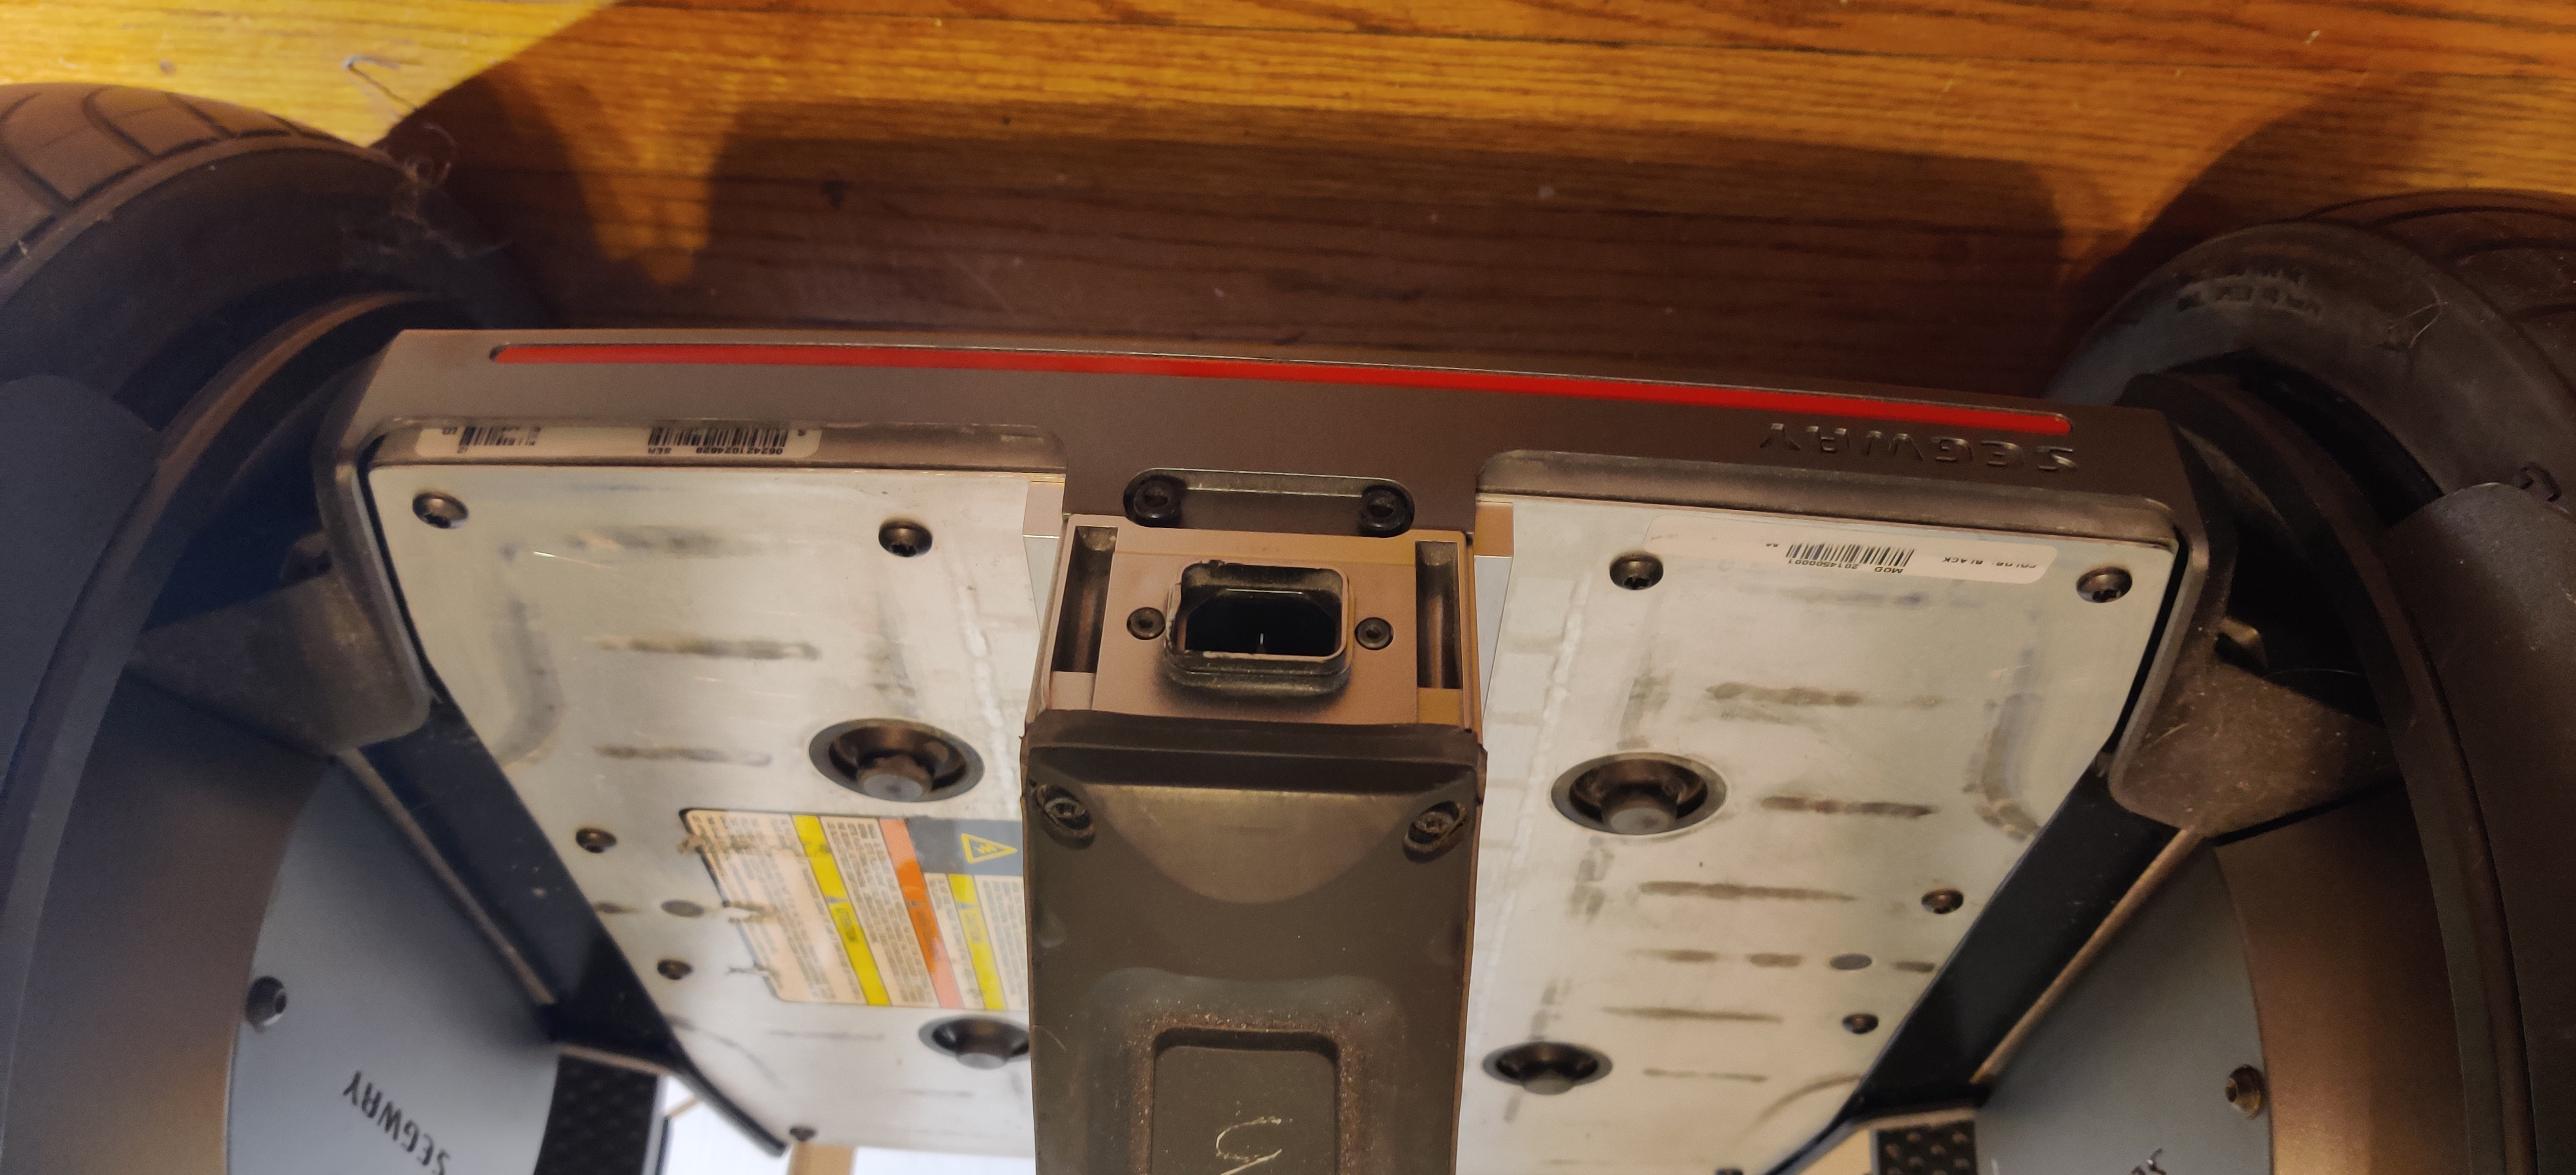
\includegraphics[]{segwayRear.jpg}
    \caption{caption}
    \label{fig:segwayRear.jpg}
\end{figure}

\begin{figure}
    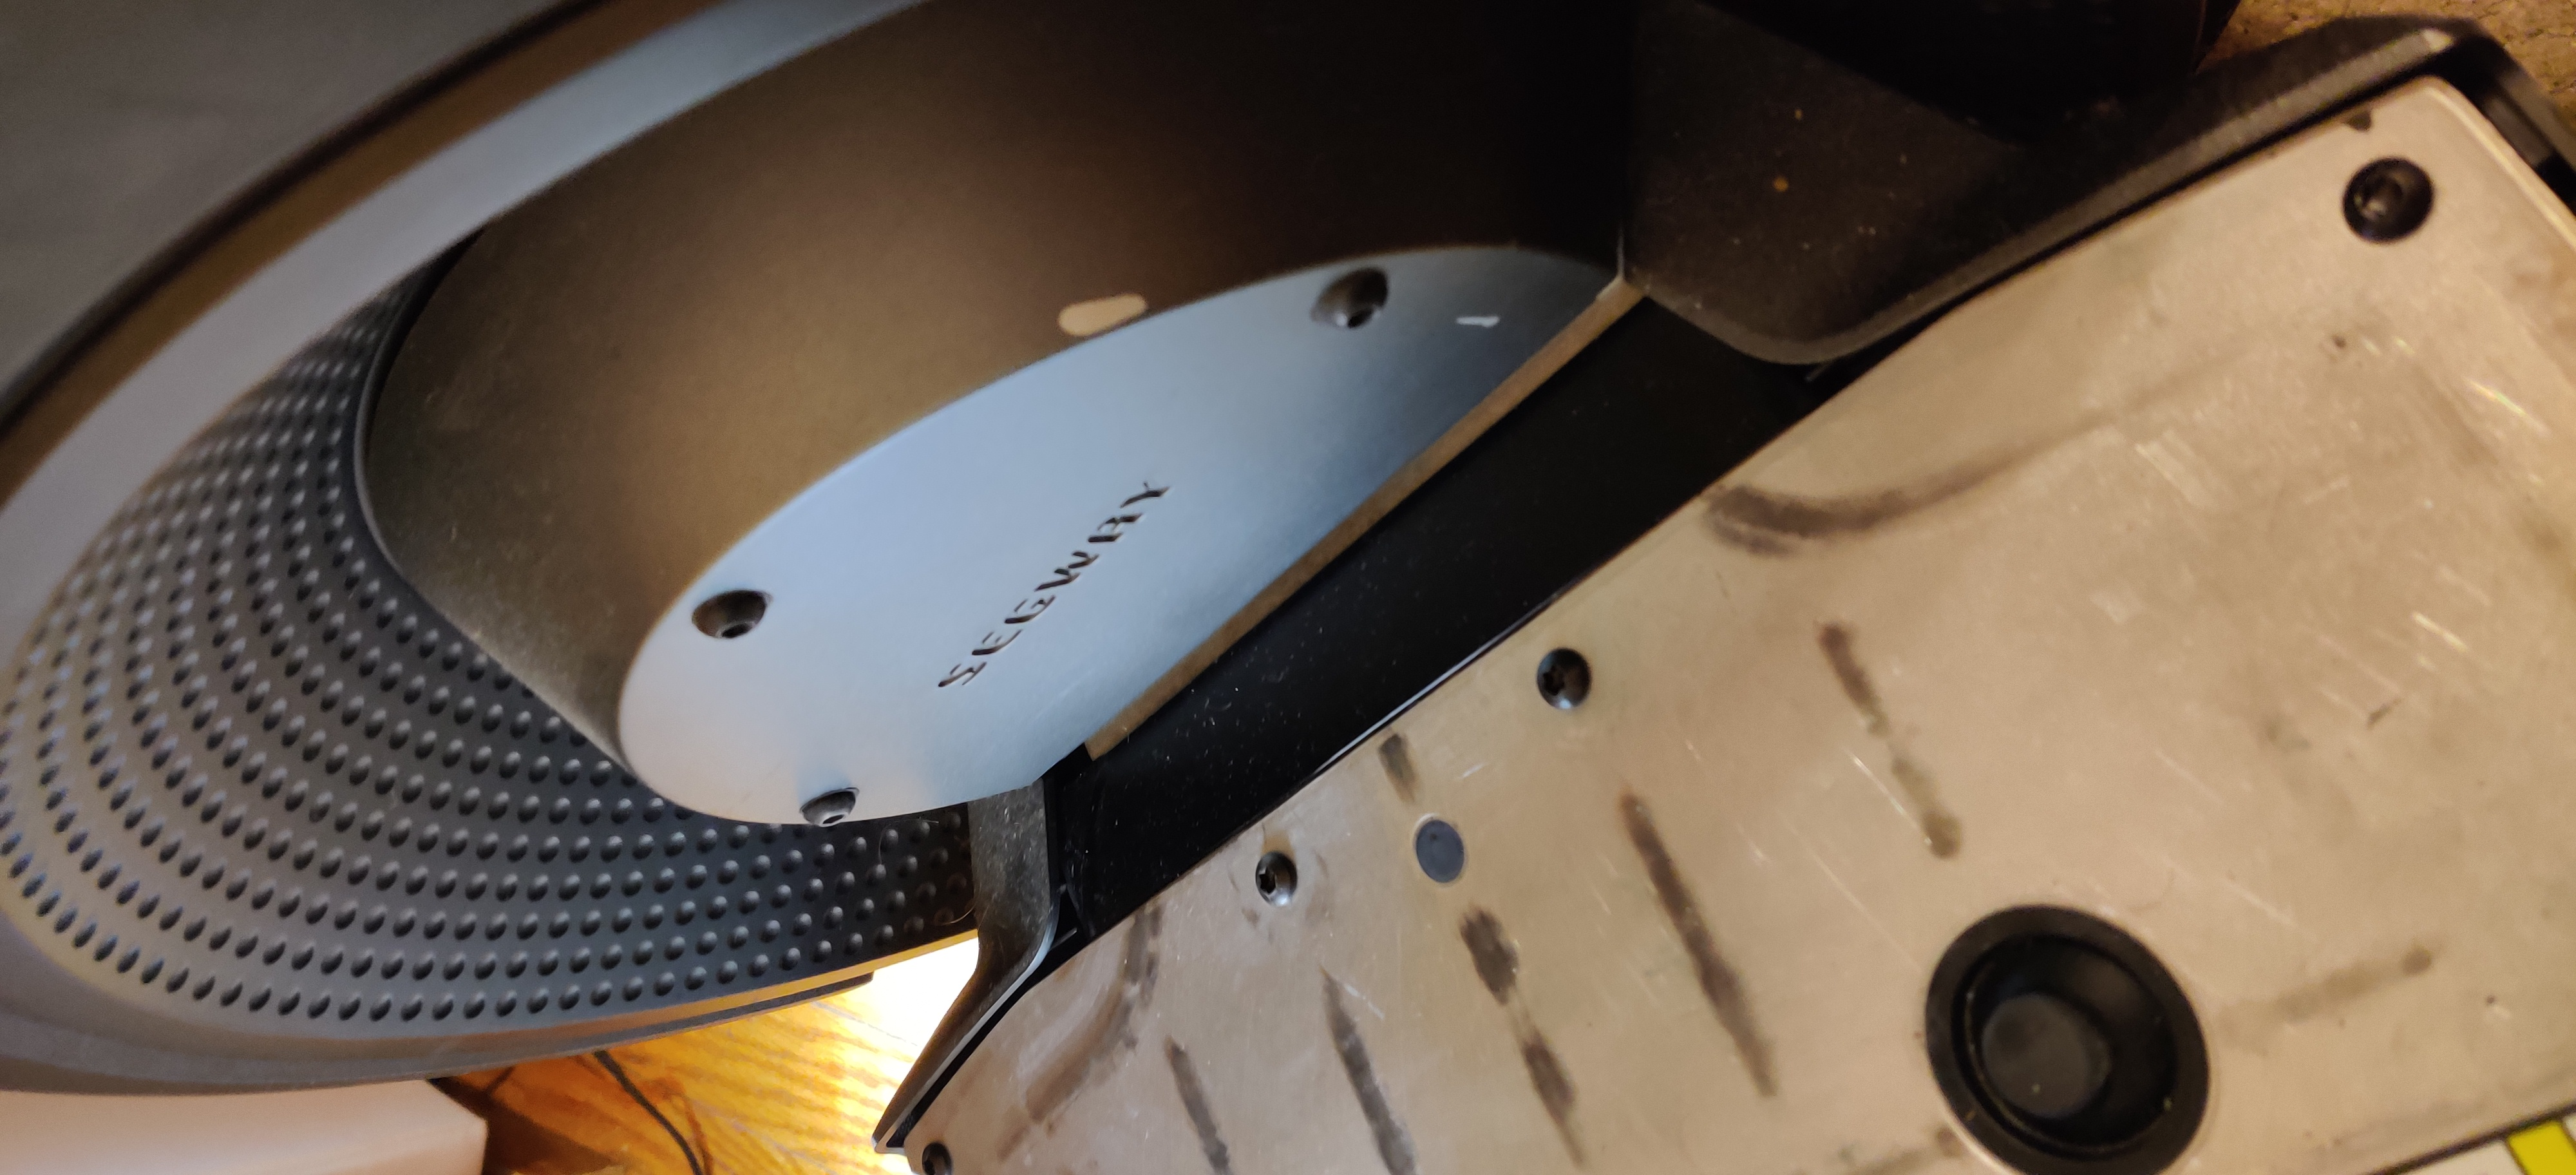
\includegraphics[]{segwayWheelAttachment.jpg}
    \caption{caption}
    \label{fig:segwayWheelAttachment.jpg}
\end{figure}

\end{document}

% References: Battery I2C protocols: https://github.com/martinbogo/pt-battery-diagnostics